\documentclass[a4paper]{article}

\def\npart {II}
\def\nterm {Michaelmas}
\def\nyear {2015}
\def\nlecturer {H. Wilton}
\def\ncourse {Algebraic Topology}
\def\nlectures {MWF.9}
\def\nnotready {}

% Imports
\ifx \nextra \undefined
  \usepackage[pdftex,
    hidelinks,
    pdfauthor={Dexter Chua},
    pdfsubject={Cambridge Maths Notes: Part \npart\ - \ncourse},
    pdftitle={Part \npart\ - \ncourse},
  pdfkeywords={Cambridge Mathematics Maths Math \npart\ \nterm\ \nyear\ \ncourse}]{hyperref}
  \title{Part \npart\ - \ncourse}
\else
  \usepackage[pdftex,
    hidelinks,
    pdfauthor={Dexter Chua},
    pdfsubject={Cambridge Maths Notes: Part \npart\ - \ncourse\ (\nextra)},
    pdftitle={Part \npart\ - \ncourse\ (\nextra)},
  pdfkeywords={Cambridge Mathematics Maths Math \npart\ \nterm\ \nyear\ \ncourse\ \nextra}]{hyperref}

  \title{Part \npart\ - \ncourse \\ {\Large \nextra}}
\fi

\author{Lectured by \nlecturer \\\small Notes taken by Dexter Chua}
\date{\nterm\ \nyear}

\usepackage{alltt}
\usepackage{amsfonts}
\usepackage{amsmath}
\usepackage{amssymb}
\usepackage{amsthm}
\usepackage{booktabs}
\usepackage{caption}
\usepackage{enumitem}
\usepackage{fancyhdr}
\usepackage{graphicx}
\usepackage{mathtools}
\usepackage{microtype}
\usepackage{multirow}
\usepackage{pdflscape}
\usepackage{pgfplots}
\usepackage{siunitx}
\usepackage{tabularx}
\usepackage{tikz}
\usepackage{tkz-euclide}
\usepackage[normalem]{ulem}
\usepackage[all]{xy}

\pgfplotsset{compat=1.12}

\pagestyle{fancyplain}
\lhead{\emph{\nouppercase{\leftmark}}}
\ifx \nextra \undefined
  \rhead{
    \ifnum\thepage=1
    \else
      \npart\ \ncourse
    \fi}
\else
  \rhead{
    \ifnum\thepage=1
    \else
      \npart\ \ncourse\ (\nextra)
    \fi}
\fi
\usetikzlibrary{arrows}
\usetikzlibrary{decorations.markings}
\usetikzlibrary{decorations.pathmorphing}
\usetikzlibrary{positioning}
\usetikzlibrary{fadings}
\usetikzlibrary{intersections}
\usetikzlibrary{cd}

\newcommand*{\Cdot}{\raisebox{-0.25ex}{\scalebox{1.5}{$\cdot$}}}
\newcommand {\pd}[2][ ]{
  \ifx #1 { }
    \frac{\partial}{\partial #2}
  \else
    \frac{\partial^{#1}}{\partial #2^{#1}}
  \fi
}

% Theorems
\theoremstyle{definition}
\newtheorem*{aim}{Aim}
\newtheorem*{axiom}{Axiom}
\newtheorem*{claim}{Claim}
\newtheorem*{cor}{Corollary}
\newtheorem*{defi}{Definition}
\newtheorem*{eg}{Example}
\newtheorem*{fact}{Fact}
\newtheorem*{law}{Law}
\newtheorem*{lemma}{Lemma}
\newtheorem*{notation}{Notation}
\newtheorem*{prop}{Proposition}
\newtheorem*{thm}{Theorem}

\renewcommand{\labelitemi}{--}
\renewcommand{\labelitemii}{$\circ$}
\renewcommand{\labelenumi}{(\roman{*})}

\let\stdsection\section
\renewcommand\section{\newpage\stdsection}

% Strike through
\def\st{\bgroup \ULdepth=-.55ex \ULset}

% Maths symbols
\newcommand{\bra}{\langle}
\newcommand{\ket}{\rangle}

\newcommand{\N}{\mathbb{N}}
\newcommand{\Z}{\mathbb{Z}}
\newcommand{\Q}{\mathbb{Q}}
\renewcommand{\H}{\mathbb{H}}
\newcommand{\R}{\mathbb{R}}
\newcommand{\C}{\mathbb{C}}
\newcommand{\Prob}{\mathbb{P}}
\renewcommand{\P}{\mathbb{P}}
\newcommand{\E}{\mathbb{E}}
\newcommand{\F}{\mathbb{F}}
\newcommand{\cU}{\mathcal{U}}
\newcommand{\RP}{\mathbb{RP}}
\newcommand{\CP}{\mathbb{CP}}

\newcommand{\ph}{\,\cdot\,}

\DeclareMathOperator{\sech}{sech}
\DeclareMathOperator{\cosech}{cosech}
\DeclareMathOperator{\cosec}{cosec}

\DeclareMathOperator{\covol}{covol}
\DeclareMathOperator{\vol}{vol}

\let\Im\relax
\let\Re\relax
\DeclareMathOperator{\Im}{Im}
\DeclareMathOperator{\Re}{Re}
\DeclareMathOperator{\im}{im}
\DeclareMathOperator{\image}{image}
\DeclareMathOperator{\Ann}{Ann}

\DeclareMathOperator*{\res}{res}
\DeclareMathOperator{\Res}{Res}
\DeclareMathOperator{\Ind}{Ind}

\DeclareMathOperator{\tr}{tr}
\DeclareMathOperator{\diag}{diag}
\DeclareMathOperator{\rank}{rank}
\DeclareMathOperator{\card}{card}
\DeclareMathOperator{\spn}{span}
\DeclareMathOperator{\adj}{adj}

\DeclareMathOperator{\erf}{erf}
\DeclareMathOperator{\erfc}{erfc}

\DeclareMathOperator{\ord}{ord}
\DeclareMathOperator{\Sym}{Sym}

\DeclareMathOperator{\sgn}{sgn}
\DeclareMathOperator{\orb}{orb}
\DeclareMathOperator{\stab}{stab}
\DeclareMathOperator{\ccl}{ccl}

\DeclareMathOperator{\lcm}{lcm}
\DeclareMathOperator{\hcf}{hcf}

\DeclareMathOperator{\Int}{Int}
\DeclareMathOperator{\id}{id}

\DeclareMathOperator{\betaD}{beta}
\DeclareMathOperator{\gammaD}{gamma}
\DeclareMathOperator{\Poisson}{Poisson}
\DeclareMathOperator{\binomial}{binomial}
\DeclareMathOperator{\multinomial}{multinomial}
\DeclareMathOperator{\Bernoulli}{Bernoulli}
\DeclareMathOperator{\like}{like}

\DeclareMathOperator{\var}{var}
\DeclareMathOperator{\cov}{cov}
\DeclareMathOperator{\bias}{bias}
\DeclareMathOperator{\mse}{mse}
\DeclareMathOperator{\corr}{corr}

\DeclareMathOperator{\otp}{otp}
\DeclareMathOperator{\dom}{dom}

\DeclareMathOperator{\Root}{Root}
\DeclareMathOperator{\supp}{supp}
\DeclareMathOperator{\rel}{rel}
\DeclareMathOperator{\Hom}{Hom}
\DeclareMathOperator{\Aut}{Aut}
\DeclareMathOperator{\Gal}{Gal}
\DeclareMathOperator{\Mat}{Mat}
\DeclareMathOperator{\End}{End}
\DeclareMathOperator{\Char}{char}
\DeclareMathOperator{\ev}{ev}
\DeclareMathOperator{\St}{St}
\DeclareMathOperator{\Lk}{Lk}
\DeclareMathOperator{\disc}{disc}
\DeclareMathOperator{\Isom}{Isom}
\DeclareMathOperator{\length}{length}
\DeclareMathOperator{\energy}{energy}
\DeclareMathOperator{\area}{area}
\DeclareMathOperator{\Syl}{Syl}
\DeclareMathOperator{\cl}{cl}
\DeclareMathOperator{\fix}{fix}

\newcommand{\GL}{\mathrm{GL}}
\newcommand{\SL}{\mathrm{SL}}
\newcommand{\PGL}{\mathrm{PGL}}
\newcommand{\PSL}{\mathrm{PSL}}
\newcommand{\PSU}{\mathrm{PSU}}
\newcommand{\Or}{\mathrm{O}}
\newcommand{\SO}{\mathrm{SO}}
\newcommand{\U}{\mathrm{U}}
\newcommand{\SU}{\mathrm{SU}}

\renewcommand{\d}{\mathrm{d}}
\newcommand{\D}{\mathrm{D}}

\tikzset{->/.style = {decoration={markings,
                                  mark=at position 1 with {\arrow[scale=2]{latex'}}},
                      postaction={decorate}}}
\tikzset{<-/.style = {decoration={markings,
                                  mark=at position 0 with {\arrowreversed[scale=2]{latex'}}},
                      postaction={decorate}}}
\tikzset{<->/.style = {decoration={markings,
                                   mark=at position 0 with {\arrowreversed[scale=2]{latex'}},
                                   mark=at position 1 with {\arrow[scale=2]{latex'}}},
                       postaction={decorate}}}
\tikzset{->-/.style = {decoration={markings,
                                   mark=at position #1 with {\arrow[scale=2]{latex'}}},
                       postaction={decorate}}}
\tikzset{-<-/.style = {decoration={markings,
                                   mark=at position #1 with {\arrowreversed[scale=2]{latex'}}},
                       postaction={decorate}}}

\tikzset{circ/.style = {fill, circle, inner sep = 0, minimum size = 3}}
\tikzset{mstate/.style={circle, draw, blue, text=black, minimum width=0.7cm}}

\definecolor{mblue}{rgb}{0.2, 0.3, 0.8}
\definecolor{morange}{rgb}{1, 0.5, 0}
\definecolor{mgreen}{rgb}{0.1, 0.4, 0.2}
\definecolor{mred}{rgb}{0.5, 0, 0}

\def\drawcirculararc(#1,#2)(#3,#4)(#5,#6){%
    \pgfmathsetmacro\cA{(#1*#1+#2*#2-#3*#3-#4*#4)/2}%
    \pgfmathsetmacro\cB{(#1*#1+#2*#2-#5*#5-#6*#6)/2}%
    \pgfmathsetmacro\cy{(\cB*(#1-#3)-\cA*(#1-#5))/%
                        ((#2-#6)*(#1-#3)-(#2-#4)*(#1-#5))}%
    \pgfmathsetmacro\cx{(\cA-\cy*(#2-#4))/(#1-#3)}%
    \pgfmathsetmacro\cr{sqrt((#1-\cx)*(#1-\cx)+(#2-\cy)*(#2-\cy))}%
    \pgfmathsetmacro\cA{atan2(#2-\cy,#1-\cx)}%
    \pgfmathsetmacro\cB{atan2(#6-\cy,#5-\cx)}%
    \pgfmathparse{\cB<\cA}%
    \ifnum\pgfmathresult=1
        \pgfmathsetmacro\cB{\cB+360}%
    \fi
    \draw (#1,#2) arc (\cA:\cB:\cr);%
}
\newcommand\getCoord[3]{\newdimen{#1}\newdimen{#2}\pgfextractx{#1}{\pgfpointanchor{#3}{center}}\pgfextracty{#2}{\pgfpointanchor{#3}{center}}}

\def\Xint#1{\mathchoice
   {\XXint\displaystyle\textstyle{#1}}%
   {\XXint\textstyle\scriptstyle{#1}}%
   {\XXint\scriptstyle\scriptscriptstyle{#1}}%
   {\XXint\scriptscriptstyle\scriptscriptstyle{#1}}%
   \!\int}
\def\XXint#1#2#3{{\setbox0=\hbox{$#1{#2#3}{\int}$}
     \vcenter{\hbox{$#2#3$}}\kern-.5\wd0}}
\def\ddashint{\Xint=}
\def\dashint{\Xint-}


\begin{document}
\maketitle
{\small
\noindent\textbf{The fundamental group}\\
Homotopy of continuous functions and homotopy equivalence between topological spaces. The fundamental group of a space, homomorphisms induced by maps of spaces, change of base point, invariance under homotopy equivalence.\hspace*{\fill} [3]

\vspace{10pt}
\noindent\textbf{Covering spaces}\\
Covering spaces and covering maps. Path-lifting and homotopy-lifting properties, and their application to the calculation of fundamental groups. The fundamental group of the circle; topological proof of the fundamental theorem of algebra. *Construction of the universal covering of a path-connected, locally simply connected space*. The correspondence between connected coverings of $X$ and conjugacy classes of subgroups of the fundamental group of $X$.\hspace*{\fill} [5]

\vspace{10pt}
\noindent\textbf{The Seifert-Van Kampen theorem}\\
Free groups, generators and relations for groups, free products with amalgamation. Statement *and proof* of the Seifert-Van Kampen theorem. Applications to the calculation of fundamental groups.\hspace*{\fill} [4]

\vspace{10pt}
\noindent\textbf{Simplicial complexes}\\
Finite simplicial complexes and subdivisions; the simplicial approximation theorem.\hspace*{\fill} [3]

\vspace{10pt}
\noindent\textbf{Homology}\\
Simplicial homology, the homology groups of a simplex and its boundary. Functorial properties for simplicial maps. *Proof of functoriality for continuous maps, and of homotopy invariance*.\hspace*{\fill} [4]

\vspace{10pt}
\noindent\textbf{Homology calculations}\\
The homology groups of $S^n$, applications including Brouwer's fixed-point theorem. The Mayer-Vietoris theorem. *Sketch of the classification of closed combinatorical surfaces*; determination of their homology groups. Rational homology groups; the Euler-Poincar\'e characteristic and the Lefschetz fixed-point theorem.\hspace*{\fill} [5]}

\tableofcontents

\setcounter{section}{-1}
\section{Introduction}
In topology, a typical problem is that we have two spaces $X$ and $Y$, and we want to know if $X\cong Y$, ie. if $X$ and $Y$ are homeomorphic. If they are homeomorphic, we can easily show this by writing down a homeomorphism. But what if they are not? How can we prove that two spaces are not homeomorphic?

For example, are $\R^m$ and $\R^n$ homeomorphic (for $m\not= n$)? Intuitively, they should not be, since they have different dimensions, and in fact they are. But how can we actually prove this?

The idea of algebraic topology is to translate these non-existence problems in topology to non-existence problems in algebra. It turns out we are much better at algebra than topology. It is \emph{much} easier to show that two groups are not isomorphic.

While the statement that $\R^m \not\cong \R^n$ for $n \not= m$ is intuitively obvious, algebraic topology can be used to prove some less obvious results.

Let $D^n$ be the $n$ dimensional unit disk, and $S^{n - 1}$ be the $n-1$ dimensional unit sphere. We will be able to show that there is no continuous map $F: D^n \to S^{n - 1}$ such that the composition
\[
  \begin{tikzcd}
    S^{n - 1} \ar[r, hook] & D^n \ar[r, "F"] & S^{n - 1}
  \end{tikzcd}
\]
is the identity, where the first arrow is the inclusion map. Alternatively, this says that we cannot continuously map the disk onto the boundary sphere such that the boundary sphere is fixed by the map.

Using algebraic topology, we can translate this statement into an algebraic statement: there is no homomorphism $F: \{0\} \to \Z$ such that
\[
  \begin{tikzcd}
    \Z \ar[r, hook] & \{0\} \ar[r, "F"] & \Z
  \end{tikzcd}
\]
is the identity. This is something we can prove in 5 seconds.

By translating a non-existence problem of a continuous map to a non-existence problem of a homomorphism, we have made our life much easier.

In algebraic topology, we will be developing a lot of machinery to do this sort of translation. However, this machinery is not easy. It will take some hard work, and will be rather tedious and boring at the beginning. So keep in mind that the point of all that hard work is to prove all these interesting theorems.

In case you are completely uninterested in topology, and don't care if $\R^m$ and $\R^n$ are homeomorphic, further applications of algebraic topology include \emph{solving equations}. For example, we will be able to prove the fundamental theorem of algebra, as well as Brouwer's fixed point theorem (which says that every continuous function from $D^2 \to D^2$ has a fixed point). If you are not interested in these as well, you may as well drop this course.

\section{Definitions}
\subsection{Some recollections and conventions}
We will start with some preliminary definitions and conventions.

\begin{defi}[Map]
  In this course, the word \emph{map} will always refer to continuous maps. We are doing topology, and never care about non-continuous functions.
\end{defi}

We are going to build a lot of continuous maps in algebraic topology. To do so, we will often need to glue maps together. The \emph{glueing lemma} tells us that this works.
\begin{lemma}[Glueing lemma]
  If $f: X\to Y$ is a function of topological spaces, $X = C\cup K$, $C$ and $K$ are both closed, then $f$ is continuous if and only if the restrictions $f|_C$ and $f|_K$are continuous.
\end{lemma}
The proof is easy from the definition of continuous maps.

\subsection{Cell complexes}
In general, we can construct some really horrible topological spaces. Even if we require them to be compact, Hausdorff etc, we can often still produce really ugly topological spaces. In algebraic topology, we will often restrict our attention to some nice topological spaces, known as \emph{cell complexes}.

To build cell complexes, we are not just glueing maps, but spaces.

\begin{defi}[Cell attachment]
  Fora a space $X$, and a map $f: S^{n - 1}\to X$, the space obtained by \emph{attaching an $n$-cell} to $X$ along $f$ is
  \[
    X\cup_{f}D^n = (X\sqcup D^N)/{\sim},
  \]
  where the equivalence relation $\sim$ is the equivalence relation generated by $x\sim f(x)$ for all $x\in S^{n - 1}\subseteq D^n$.

  Intuitively, a map $f: S^{n - 1}\to X$ is just picks out a subset $X$ that looks like the sphere. So we are just sticking a disk onto $X$ by attaching the boundary of the disk onto a sphere within $X$.
  \begin{center}
    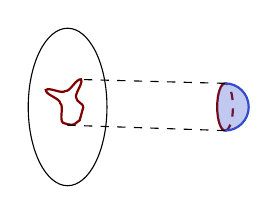
\begin{tikzpicture}
      \draw ellipse (0.5 and 1);

      \draw [thick, mred, decorate, decoration={snake}] circle [radius=0.2];

      \draw [thick, mred] (2, 0.3) arc (90:270:0.1 and 0.3);
      \draw [dashed, thick, mred] (2, -0.3) arc (270:450:0.1 and 0.3);

      \fill [mblue, opacity=0.3] (2, 0.3) arc (90:270:0.1 and 0.3) arc (270:450:0.3);
      \draw [thick, mblue] (2, -0.3) arc (270:450:0.3);

      \draw [dashed] (2, 0.3) -- (0.12, 0.35);
      \draw [dashed] (2, -0.3) -- (-0.05, -0.23);
    \end{tikzpicture}
  \end{center}
\end{defi}

\begin{defi}[Cell complex]
  A (finite) \emph{cell complex} is a space $X$ obtained by
  \begin{enumerate}
    \item Start with a discrete finite set $X^{(0)}$.
      \begin{center}
        \begin{tikzpicture}
          \node [circ] at (0, 0) {};
          \node [circ] at (-1, -1.2) {};
          \node [circ] at (1, -1) {};
          \node [circ] at (0.3, -2) {};
        \end{tikzpicture}
      \end{center}
    \item Given $X^{n - 1}$, for $X^n$ by taking a finite set of maps $\{f_\alpha: S^{n - 1} \to X^{(n - 1)}\}$  by attaching $n$-cells along the $f_\alpha$:
      \[
        X^{(n)} = \left(X^{(n - 1)}\sqcup \bigsqcup_\alpha D_{\alpha}^N\right)/\{x\sim f_\alpha(x)\}.
      \]
      For example, given the $X^{(0)}$ above, we can attach some loops and lines to obtain the following $X^{(1)}$
      \begin{center}
        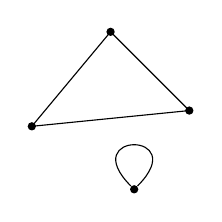
\begin{tikzpicture}
          \node [circ] at (0, 0) {};
          \node [circ] at (-1, -1.2) {};
          \node [circ] at (1, -1) {};
          \node [circ] (3) at (0.3, -2) {};

          \draw (0, 0) -- (-1, -1.2) -- (1, -1) -- (0, 0);
          \draw (3) edge [loop, looseness=30] (3);
        \end{tikzpicture}
      \end{center}
      We can add surfaces to obtain the following $X^{(2)}$
      \begin{center}
        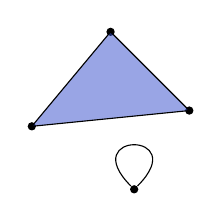
\begin{tikzpicture}
          \node [circ] at (0, 0) {};
          \node [circ] at (-1, -1.2) {};
          \node [circ] at (1, -1) {};
          \node [circ] (3) at (0.3, -2) {};

          \draw [fill = mblue, fill opacity=0.5] (0, 0) -- (-1, -1.2) -- (1, -1) -- (0, 0);
          \draw (3) edge [loop, looseness=30] (3);
        \end{tikzpicture}
      \end{center}
    \item Stop at some $X = X^{(k)}$. The minimum such $k$ is the \emph{dimension} of $X$.
  \end{enumerate}
  To define non-finite cell complexes, we just have to remove the words ``finite'' in the definition and remove the final condition.
\end{defi}

\begin{eg}
  The following is \emph{not} a cell complex: we take $\R^2$, and add a circle with radius $\frac{1}{2}$ and center $(0, \frac{1}{2})$. Then we add another circle with radius $\frac{1}{4}$ and center $(0, \frac{1}{4})$, then a circle with radius $\frac{1}{8}$ and center $(0, \frac{1}{8})$ etc. We obtain something like
  \begin{center}
    \begin{tikzpicture}[scale=2]
      \draw (0, 0.5) circle [radius=0.5];
      \draw (0, 0.25) circle [radius=0.25];
      \draw (0, 0.125) circle [radius = 0.125];
      \draw (0, 0.0625) circle [radius = 0.0625];
      \draw [gray] (-2, 0) -- (2, 0);

      \node [circ, mblue] at (0, 1) {};
      \node [circ, mblue] at (0, 0.5) {};
      \node [circ, mblue] at (0, 0.25) {};
      \node [circ, mblue] at (0, 0.125) {};
    \end{tikzpicture}
  \end{center}
  This is known as the \emph{Hawaiian Earring}.

  Why is this not an (infinite) cell complex? We did obtain it by attaching 1-cells to the single point $(0, 0)$. However, when attaching cells to a cell complex, the cells should not be ``close'' to each other. They are completely separated from each other apart from touching at the origin. However, here the circles clump together at the origin.

  In particular, if we take the following sequence $(0, 1), (0, \frac{1}{2}), (0, \frac{1}{4}), \cdots$, it converges to $(0, 0)$. If this were a cell complex, then this shouldn't happen because the cells are unrelated, and picking a point from each cell should not produce a convergent sequence (if you are not convinced, if we actually did produce by attaching cells, then note that during the attaching process, we needn't have attached them this way. We could have made it such that the $n$th cell has radius $n$. Then clearly picking the topmost point of each cell will not produce a convergent sequence).

  We will see that the Hawaiian Earring will be a counterexample to a lot of our theorems here.
\end{eg}

\section{Homotopy and the fundamental group}
This will be our first trick to translate topological spaces into groups.

\setcounter{subsection}{-1}
\subsection{Motivation}
Recall that we wanted to prove that $\R^n \not\cong \R^m$ for $n\not= m$. Let's first do the simple case, where $m = 1, n = 2$. We want to show that $\R\not\cong \R^2$.

This is not hard. We know that $\R$ is a line, while $\R^2$ is a plane. Let's try to remove a point from each of them.  If we remove a point from $\R$, the space stops being path connected. However, removing a point does not have this effect on $\R^2$. Since being path connected is a topological property, we have now showed that $\R$ and $\R^2$ are not homeomorphic.

Unfortunately, this does not extend very far. We cannot use this to show that $\R^2$ and $\R^3$ are not homeomorphic. What else can we do?

Notice that when we remove a point from $\R^2$, sure it is still connected, but something has changed.

Consider a circle containing the origin in $\R^2 \setminus \{0\}$. If the origin were there, we can keep shrinking the circle down until it becomes a point. However, we cannot do this if the origin is missing.
\begin{center}
  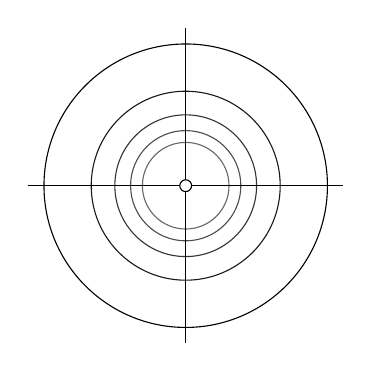
\begin{tikzpicture}
    \draw (-2, 0) -- (2, 0);
    \draw (0, -2) -- (0, 2);

    \draw [fill=white] circle [radius=0.075];
    \draw circle [radius=1.8];
    \draw [opacity=0.9] circle [radius=1.2];
    \draw [opacity=0.8] circle [radius=0.9];
    \draw [opacity=0.7] circle [radius=0.7];
    \draw [opacity=0.6] circle [radius=0.55];
  \end{tikzpicture}
\end{center}
The strategy now is to exploit the fact that $\R^2 \setminus \{0\}$ has circles which cannot be deformed to points.

\subsection{Homotopy}
We have just talked about the notion of ``deforming'' circles to a point. We can think of a circle in $X$ as a map $S^1 \to X$, and we want to ``deform'' this map to a point. This process of deformation is known as \emph{homotopy}. Here we are going to use the interval $[0, 1]\subseteq \R $ a lot, and we will just call it $I$.
\begin{notation}
  \[
    I = [0, 1]\subseteq \R.
  \]
\end{notation}

\begin{defi}[Homotopy]
  Let $f, g: X\to Y$ be maps. A \emph{homotopy} from $f$ to $g$ is a map
  \[
    H: X\times I \to Y
  \]
  such that
  \[
    H(x, 0) = f(x),\quad H(x, 1) = g(x).
  \]
  We think of the interval $I$ as time. For each time $t$, $H(\cdot, t)$ defines a map $X\to Y$. So we want to start from $f$, move with time, and eventually reach $g$.

  If such an $H$ exists, we say $f$ is \emph{homotopic} to $g$, and write $f\simeq g$. If we want to make it explicit that the homotopy is $H$, we write $f \simeq_H g$.
\end{defi}
As mentioned at the beginning, by calling $H$ a map, we are requiring it to be continuous.

Sometimes, we don't want a general homotopy. We might want to make sure that when we are deforming from a path $f$ to $g$, the end points of the path don't move. In general, we have
\begin{defi}[Homotopy $\rel$ A]
  $f$ is \emph{homotopic to} $g$ \emph{rel} $A$, written $f\simeq g\rel A$, if for all $a \in A\subseteq X$, we have
  \[
    H(a, t) = f(a) = g(a).
  \]
\end{defi}
This notion will find itself useful later, but we don't have to pay too much attention to this yet.

Our notation suggests that homotopy is an equivalence relation. Indeed, we have
\begin{prop}
  For spaces $X, Y$, and $A\subseteq X$, the ``homotopic $\rel A$'' relation is an equivalence relation. In particular, when $A = \emptyset$, homotopy is an equivalence relation.
\end{prop}

\begin{proof}\leavevmode
  \begin{enumerate}
    \item Reflexivity: $f \simeq f$ since $H(x, t) = f(x)$ is a homotopy.
    \item Symmetry: is $H(x, t)$ is a homotopy from $f$ to $g$, then $H(x, 1 - t)$ is a homotopy from $g$ to $h$.
    \item Transitivity: Suppose $f, g, h: X\to Y$ and $f\simeq_H g\rel A$, $g\simeq_{H'} h \rel A$. We want to show that $f\simeq h \rel A$. The idea is to ``glue'' the two maps together.

      We know how to continuously deform $f$ to $g$, and from $g$ to $h$. So we just do these one after another.
      We define $H'': X\times I \to Y$ by
      \[
        H(x, t) =
        \begin{cases}
          H(x, 2t) & 0 \leq t \leq \frac{1}{2}\\
          H'(x, 2t - 1) & \frac{1}{2} \leq t \leq 1
        \end{cases}
      \]
      This is well-defined since $H(x, 1) = g(x) = H'(x, 0)$. This is also continuous by the gluing lemma. It is easy to check that $H''$ is a homotopy $\rel A$.
  \end{enumerate}
\end{proof}

We now have a notion of equivalence of maps --- two maps are equivalent if they are homotopic. We can extend the notion of homotopy to spaces as well.

Recall that when we defined homeomorphism, we required that there is some $f, g$ such that $f\circ g = \id$, $g\circ f = \id$. Here, we replace equality by homotopy.
\begin{defi}[Homotopy equivalence]
  A map $f: X\to Y$ is a \emph{homotopy equivalence} if there exists a $g: Y\to X$ such that $f\circ g \simeq \id_Y$ and $g\circ f \simeq \id_X$. We call $g$ a \emph{homotopy inverse} for $f$.

  If a homotopy equivalence $f: X\to Y$ exists, we say that $X$ and $Y$ are homotopy equivalent and write $X\simeq Y$.
\end{defi}
We are soon going to prove that this is indeed an equivalence relation on spaces, but we first look at some examples of homotopy equivalent spaces. Clearly, homeomorphic spaces are homotopy equivalent. However, we will see that we can do much more ``violent'' things to a space and still be homotopy equivalent.
\begin{eg}
  Let $X = S^1$, $Y = \R^2 \setminus \{0\}$. We have a natural inclusion map $i: X\hookrightarrow Y$. To obtain a map $Y \to X$, we can project each point onto the circle.
  \begin{center}
    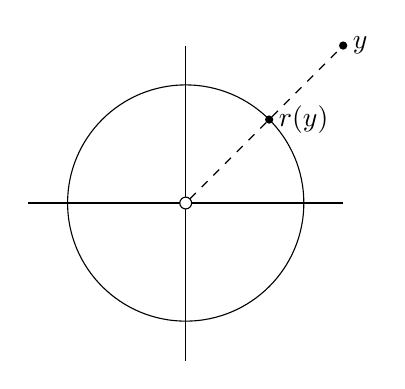
\begin{tikzpicture}
      \draw (-2, 0) -- (2, 0);
      \draw (0, -2) -- (0, 2);

      \draw [fill=white] circle [radius=0.075];
      \draw circle [radius=1.5];

      \node [circ] at (1.06, 1.06) {};
      \node [circ] at (2, 2) {};
      \node at (1.06, 1.06) [right] {$r(y)$};
      \node at (2, 2) [right] {$y$};
      \draw [dashed] (0.053, 0.053) -- (2, 2);
    \end{tikzpicture}
  \end{center}
  In particular, we define $r: Y\to X$ by
  \[
    r(y) = \frac{y}{\|y\|}.
  \]
  We immediately have $r\circ i = \id_X$. We will now see that $i\circ r \simeq \id_Y$. The composition $i\circ r$ first projects each object into $S^1$, and then includes it back into $\R^2 \setminus \{0\}$. So this is just the projection map. We can define a homotopy $H: Y\times I \to Y$ by
  \[
    H(y, t) = \frac{y}{t + (1 - t)\|y\|}.
  \]
  This is continuous, and $H(\cdot, 0) = i\circ r$, $H(\cdot, 1) = \id_Y$.
\end{eg}
As we have said, homotopy equivalence can do really ``violent'' things to a space. We started with a 2-dimensional $\R^2\setminus \{0\}$ space, and squashed it into a one-dimensional sphere.

Hence we see that homotopy doesn't \emph{care} about dimensions. This seems to be a rather fundamental thing in geometry, and we are discarding it. So what is left? What does homotopy preserve?

While $S^1$ and $\R^2 \setminus \{0\}$ seem rather different, they have something in common --- they both have a ``hole''. We will later see that this is what homotopy preserves.

\begin{eg}
  Let $Y = \R^n$, $X = \{0\} = *$. Let $X\hookrightarrow Y$ be the inclusion map, and $r: Y\to X$ be the unique map that sends everything to $\{0\}$. Again, we have $r\circ i = \id_X$. We can also obtain a homotopy from $i \circ r$ to $\id_Y$ by
  \[
    H(y, t) = ty.
  \]
\end{eg}
Again, from the point of view of homotopy theory, $\R^n$ is just the same as a point! You might think that this is something crazy to do --- we have just given up a lot of structure of topological spaces. However, this turns out to be a really useful notion.

In general things homotopic to a single point are known as \emph{contractible spaces}.
\begin{notation}
  $*$ denotes the one-point space $\{0\}$.
\end{notation}

\begin{defi}[Contractible space]
  If $X\simeq *$, then $X$ is \emph{contractible}.
\end{defi}

We now show that homotopy of spaces is an equivalence relation. To do this, we first need a lemma.
\begin{lemma}
  Consider the spaces and arrows
  \[
    \begin{tikzcd}
      X \ar[r, bend left, "f_0"] \ar[r, bend right, "f_1"'] & Y \ar[r, bend left, "g_0"] \ar[r, bend right, "g_1"'] & Z
    \end{tikzcd}
  \]
  If $f_0\simeq_H f_1$ and $g_0\simeq_{H'} g_1$, then $g_0\circ f_0 \simeq g_1 \circ f_1$.
\end{lemma}

\begin{proof}
  We will show that $g_0 \circ f_0 \simeq g_0 \circ f_1 \simeq g_1 \circ f_1$. Then we are done since homotopy between maps is an equivalence relation. So we need to write down two homotopies.

  \begin{enumerate}
    \item Consider the following composition:
      \[
        \begin{tikzcd}
          X\times I \ar[r, "H"] & Y \ar[r, "g_0"] & Z
        \end{tikzcd}
      \]
      It is easy to check that this is the first homotopy we need to show $g_0\circ f_0 = g_0 \circ f_1$.
    \item The following composition is a homotopy from $g_0 \circ f_1$ to $g_1 \circ f_1$:
      \[
        \begin{tikzcd}
          X\times I \ar[r, "f_1\times \id_I"] & Y\times I \ar[r, "H'"] & Z
        \end{tikzcd}
      \]
  \end{enumerate}
\end{proof}

\begin{prop}
  Homotopy on spaces is a equivalence relation.
\end{prop}

\begin{proof}(sketch)
  Symmetry and reflexivity are trivial, and applying the previous lemma several times can show transitivity.
\end{proof}

\begin{defi}[Retraction]
  Let $A\subseteq X$ be a subspace. A \emph{retraction} $r: X\to A$ is a map such that $r\circ i = \id_A$, where $i: A\hookrightarrow X$ is the inclusion.
\end{defi}
This map sends everything in $X$ to $A$ without mmoving things in $A$. Roughly speaking, if such a retraction exists, then $A$ is no more complicated than $X$.

\begin{defi}{Deformation retraction}
  The retraction $r$ is a \emph{deformation retraction} if $i\circ r \simeq \id_X$. Some authors requires that this homotopy is a homotopy rel $A$.
\end{defi}
Roughly, this says that $A$ is as complicated as $X$.

\begin{eg}
Take $X$ any space, and $A = \{x\}\subseteq X$. Then the constant map $r: X\to A$ is a retraction. If $X$ is contractible, then this is a deformation retract.
\end{eg}

\subsection{Paths}
\begin{defi}[Path]
  A \emph{path} in a space $X$ is a map $\gamma: I\to X$. If $\gamma(0) = x_0$ and $\gamma(1) = x_1$, we say $\gamma$ is a path from $x_0$ to $x_1$, and write $\gamma: x_0 \rightsquigarrow x_1$.

  If $\gamma(0) = \gamma(1)$, then $\gamma$ is called a \emph{loop} (based at $x_0$).
  \begin{center}
    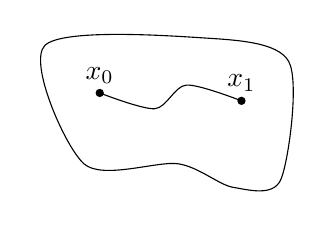
\begin{tikzpicture}
      \draw plot [smooth cycle] coordinates {(-1.2, -0.7) (0, -0.7) (0.7, -1) (1.3, -0.9) (1.4, 0.6) (0.3, 0.9) (-1.7, 0.8)};

      \node [circ] at (-1, 0.2) {};
      \node [above] at (-1, 0.2) {$x_0$};
      \node [circ] at (0.8, 0.1) {};
      \node [above] at (0.8, 0.1) {$x_1$};
      \draw plot [smooth] coordinates {(-1, 0.2) (-0.3, 0) (0.1, 0.3) (0.8, 0.1)};
    \end{tikzpicture}
  \end{center}
\end{defi}
Note that this map does not have to be injective. It can be self intersecting or do all sorts of weird stuff.

Recall that the basic idea of algebraic topology is to assign to each space $X$ an (algebraic) object, which is (hopefully) easier to deal with. In homotopy theory, we do so using the idea of paths.

To do so, we need to be able to perform operations on paths.
\begin{defi}[Concatenation of paths]
  If we have two paths $\gamma_1$ from $x_0$ to $x_1$; and $\gamma_2$ from $x_1$ to $x_2$, we define the \emph{concatenation to be}
  \[
    (\gamma_1\cdot \gamma_2)(t) =
    \begin{cases}
      \gamma(2t) & 0 \leq t \leq \frac{1}{2}\\
      \gamma(2t - 1) & \frac{1}{2} \leq t \leq 1.
    \end{cases}
  \]
  This is continuous by the gluing lemma.
\end{defi}
Note that we concatenate left to right, but function composition goes from right to left.
\begin{center}
  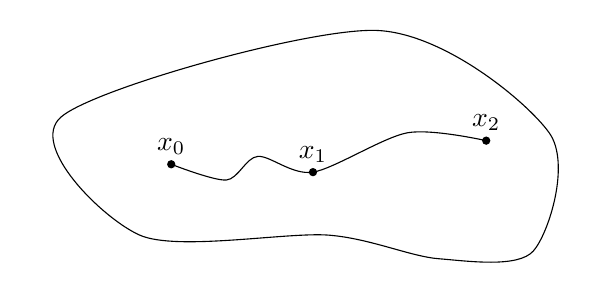
\begin{tikzpicture}
    \draw plot [smooth cycle] coordinates {(-2.4, -0.7) (0, -0.7) (1.4, -1) (2.6, -0.9) (2.8, 0.6) (0.6, 1.9) (-3.4, 0.8)};

    \node [circ] at (-2, 0.2) {};
    \node [above] at (-2, 0.2) {$x_0$};
    \node [circ] at (-0.2, 0.1) {};
    \node [above] at (-0.2, 0.1) {$x_1$};
    \node [circ] at (2, 0.5) {};
    \node [above] at (2, 0.5) {$x_2$};
    \draw plot [smooth] coordinates {(-2, 0.2) (-1.3, 0) (-0.9, 0.3) (-0.2, 0.1) (1, 0.6) (2, 0.5)};
  \end{tikzpicture}
\end{center}
\begin{defi}[Inverse of path]
  The \emph{inverse} of path $\gamma: I \to X$ is defined by
  \[
    \gamma^{-1}(t) = \gamma(1 - t).
  \]
  This is exactly the same path but going in the opposite direction.
\end{defi}

What else do we need? We need an identity.
\begin{defi}[Constant path]
  The \emph{constant path} at a point $x\in X$ is given by $c_x(t) = x$.
\end{defi}

We haven't actually got a good algebraic system. We have $\gamma$ and $\gamma^{-1}$, but when we compose them, we get a path from $x_1$ to $x_2$ and back, and not the identity. Also, we are not able to combine arbitrary paths in a space.

Before we make these into proper algebraic operations, we will talk bout something slightly different.

\begin{defi}[Path components]
  We can define a relation on $X$: $x_1 \sim x_2$ if there exists path from $x_1$ to $x_2$. By the concatenation, inverse and constant paths, $\sim$ is an equivalence relation. The equivalence classes $[x]$ are called \emph{path components}. We denote the quotient $X/{\sim}$ by $\pi_0(X)$.
\end{defi}
\begin{center}
  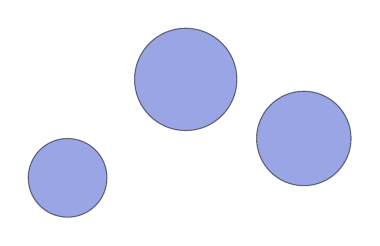
\begin{tikzpicture}[scale=0.5]
    \draw [fill=mblue, opacity=0.5] circle [radius = 1];
    \draw (3, 2.5) [fill=mblue, opacity=0.5] circle [radius = 1.3];
    \draw (6, 1) [fill=mblue, opacity=0.5] circle [radius = 1.2];
  \end{tikzpicture}
\end{center}
In the above space, we have three path components.

This isn't really a very useful definition, since most spaces we care about are path-connected, ie. only have one path component. However, this is a first step at associating \emph{something} to spaces. We can view this as a ``toy model'' for the more useful definitions we will later have.

One important property of this $\pi_0$ is that not only does it associate a set to each topological space, but also associates a function between the corresponding sets to each continuous map.
\begin{prop}
  For any map $f: X\to Y$, there is a well-defined function
  \[
    \pi_0(f): \pi_0(X) \to \pi_0(Y),
  \]
  defined by
  \[
    \pi_0(f)([x]) = [f(x)].
  \]
  Furthermore,
  \begin{enumerate}
    \item If $f\sim g$, then $\pi_0(f) = \pi_0(g)$.
    \item For any maps $\begin{tikzcd} A \ar[r, "h"] & B\ar[r, "k"] & C\end{tikzcd}$, we have $\pi_0(k\circ h) = \pi_0(k)\circ \pi_0 (h)$.
    \item $\pi_0(\id_X) = \id_{\pi_0(x)}$
  \end{enumerate}
\end{prop}
Proof is left as an easy exercise.

\begin{cor}
  If $f: X\to Y$ is a homotopy equivalence, then $\pi_0(f)$ is a bijection.
\end{cor}

\begin{eg}
  The two point space $X = \{-1, 1\}$ is not contractible. Because $|\pi_0(X)|$, but $|\pi_0(*)| = 1$.
\end{eg}
This is a rather silly example, since we can easily prove it directly. However, this is an example to show how we can use these machinery to prove topological results.

Now let's return to our operations on paths, and try to make them algebraic.

\begin{defi}[Homotopy of paths]
  Paths $\gamma, \gamma': I\to X$ are \emph{homotopic as paths} if they are homotopic rel $\{0, 1\}\subseteq I$, ie. the end points are fixed. We write $\gamma\simeq \gamma'$.
\end{defi}
\begin{center}
  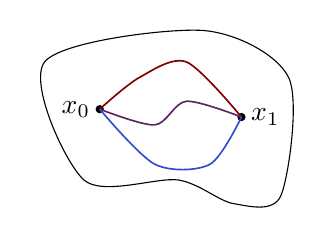
\begin{tikzpicture}
    \draw plot [smooth cycle] coordinates {(-1.2, -0.7) (0, -0.7) (0.7, -1) (1.3, -0.9) (1.4, 0.6) (0.3, 1.2) (-1.7, 0.8)};

    \node [circ] at (-1, 0.2) {};
    \node [left] at (-1, 0.2) {$x_0$};
    \node [circ] at (0.8, 0.1) {};
    \node [right] at (0.8, 0.1) {$x_1$};
    \draw [semithick, mred] plot [smooth] coordinates {(-1, 0.2) (-0.5, 0.6) (0.1, 0.8) (0.8, 0.1)};
    \draw [semithick, mred!50!mblue] plot [smooth] coordinates {(-1, 0.2) (-0.3, 0) (0.1, 0.3) (0.8, 0.1)};
    \draw [semithick, mblue] plot [smooth] coordinates {(-1, 0.2) (-0.3, -0.5) (0.4, -0.5) (0.8, 0.1)};
  \end{tikzpicture}
\end{center}
Note that we would necessarily want to fix the two end points. Otherwise, if we allow end points to move, we can shrink any path into a constant path, and our definition of homotopy would be rather silly.

This homotopy works well with our previous operations on paths.
\begin{prop}
  Let $\gamma_1, \gamma_2: I \to X$ be paths, $\gamma_1(1) = \gamma_2(0)$. Then if $\gamma_1\simeq \gamma_1'$ and $\gamma_2 \simeq \gamma_2'$, then $\gamma_1 \cdot \gamma_2 \simeq \gamma_1' \cdot \gamma_2'$.
\end{prop}
\begin{center}
  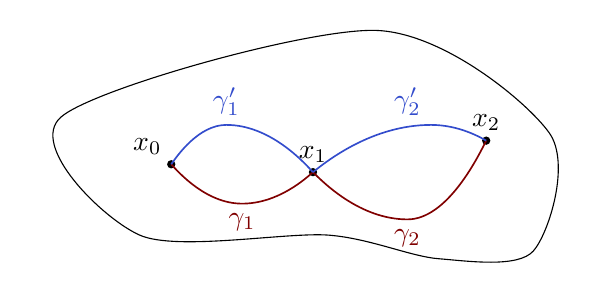
\begin{tikzpicture}
    \draw plot [smooth cycle] coordinates {(-2.4, -0.7) (0, -0.7) (1.4, -1) (2.6, -0.9) (2.8, 0.6) (0.6, 1.9) (-3.4, 0.8)};

    \node [circ] at (-2, 0.2) {};
    \node [anchor = south east] at (-2, 0.2) {$x_0$};
    \node [circ] at (-0.2, 0.1) {};
    \node [above] at (-0.2, 0.1) {$x_1$};
    \node [circ] at (2, 0.5) {};
    \node [above] at (2, 0.5) {$x_2$};
    \draw [semithick, mred] (-2, 0.2) parabola bend (-1.1, -0.3) (-0.2, 0.1);
    \draw [semithick, mred] (-0.2, 0.1) parabola bend (1, -0.5) (2, 0.5);

    \draw [semithick, mblue] (-2, 0.2) parabola bend (-1.3, 0.7) (-0.2, 0.1);
    \draw [semithick, mblue] (-0.2, 0.1) parabola bend (1.3, 0.7) (2, 0.5);

    \node [mred, below] at (-1.1, -0.3) {$\gamma_1$};
    \node [mred, below] at (1, -0.5) {$\gamma_2$};

    \node [mblue, above] at (-1.3, 0.7) {$\gamma_1'$};
    \node [mblue, above] at (1, 0.7) {$\gamma_2'$};
  \end{tikzpicture}
\end{center}

\begin{proof}
  Suppose that $\gamma_1 \simeq_{H_1}\gamma_1'$ and $\gamma_2\simeq_{H_2}\gamma_2'$. Then we have the diagram
  \begin{center}
    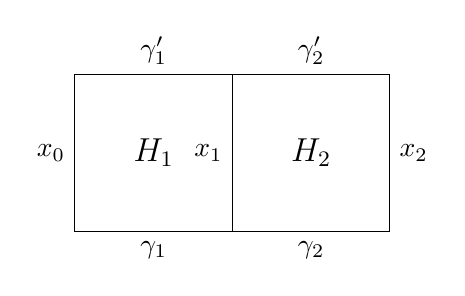
\begin{tikzpicture}
      \draw (0, 0) rectangle (2, 2);
      \draw (2, 0) rectangle (4, 2);
      \node at (1, 0) [below] {$\gamma_1$};
      \node at (3, 0) [below] {$\gamma_2$};
      \node at (1, 2) [above] {$\gamma_1'$};
      \node at (3, 2) [above] {$\gamma_2'$};
      \node at (0, 1) [left] {$x_0$};
      \node at (2, 1) [left] {$x_1$};
      \node at (4, 1) [right] {$x_2$};

      \node at (1, 1) {\large $H_1$};
      \node at (3, 1) {\large $H_2$};
    \end{tikzpicture}
  \end{center}
  We can thus construct a homotopy by
  \[
    H(s, t) =
    \begin{cases}
      H_1(s, 2t) & 0 \leq t \leq \frac{1}{2}\\
      H_2(s, 2t - 1) & \frac{1}{2} \leq t \leq 1
    \end{cases}.
  \]
\end{proof}

To solve all our previous problems about operations on paths not behaving well, we can look at paths \emph{up to homotopy}.
\begin{prop}
  Let $\gamma_0: x_0 \leadsto x_1, \gamma_1: x_1 \leadsto x_2, \gamma_2: x_2 \leadsto x_3$ be paths. Then
  \begin{enumerate}
    \item $(\gamma_0 \cdot \gamma_1)\cdot \gamma_2 \simeq \gamma_0 \cdot (\gamma_1\cdot \gamma_2)$
    \item $\gamma_0 \cdot c_{x_1}\simeq \gamma_0 \simeq c_{x_0}\cdot \gamma_0$.
    \item $\gamma_0 \cdot \gamma_0^{-1}\simeq c_{x_0}$ and $\gamma_0^{-1}\cdot \gamma_0 \simeq c_{x_1}$.
  \end{enumerate}
\end{prop}

\begin{proof}\leavevmode
  \begin{enumerate}
    \item Consider the following diagram:
      \begin{center}
        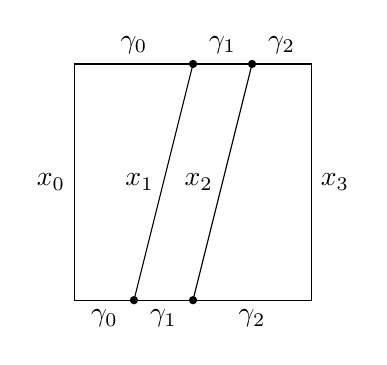
\begin{tikzpicture}[scale=0.75]
          \draw rectangle (4, 4);

          \node at (0, 2) [left] {$x_0$};
          \node at (4, 2) [right] {$x_3$};

          \node [circ] at (1, 0) {};
          \node [circ] at (2, 0) {};
          \node [circ] at (2, 4) {};
          \node [circ] at (3, 4) {};

          \node [below] at (0.5, 0) {$\gamma_0$};
          \node [below] at (1.5, 0) {$\gamma_1$};
          \node [below] at (3, 0) {$\gamma_2$};

          \node [above] at (1, 4) {$\gamma_0$};
          \node [above] at (2.5, 4) {$\gamma_1$};
          \node [above] at (3.5, 4) {$\gamma_2$};

          \draw (1, 0) -- (2, 4) node [pos=0.5, left] {$x_1$};
          \draw (2, 0) -- (3, 4) node [pos=0.5, left] {$x_2$};
        \end{tikzpicture}
      \end{center}
    \item Consider the following diagram:
      \begin{center}
        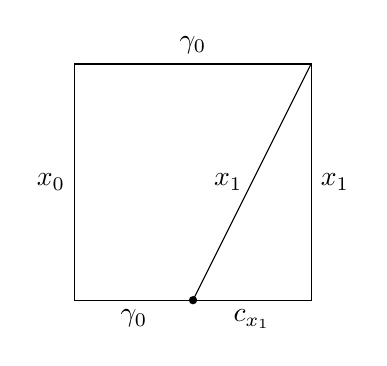
\begin{tikzpicture}[scale=0.75]
          \draw rectangle (4, 4);
          \node [circ] at (2, 0) {};
          \node at (1, 0) [below] {$\gamma_0$};
          \node at (3, 0) [below] {$c_{x_1}$};
          \node at (2, 4) [above] {$\gamma_0$};
          \node at (0, 2) [left] {$x_0$};
          \node at (4, 2) [right] {$x_1$};

          \draw (2, 0) -- (4, 4) node [pos=0.5, left] {$x_1$};
        \end{tikzpicture}
      \end{center}
    \item Consider the following diagram:
      \begin{center}
        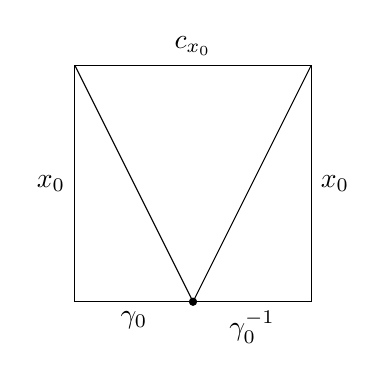
\begin{tikzpicture}[scale=0.75]
          \draw rectangle (4, 4);
          \node [circ] at (2, 0) {};
          \node at (1, 0) [below] {$\gamma_0$};
          \node at (3, 0) [below] {$\gamma_0^{-1}$};
          \node at (2, 4) [above] {$c_{x_0}$};
          \node at (0, 2) [left] {$x_0$};
          \node at (4, 2) [right] {$x_0$};

          \draw (0, 4) -- (2, 0) -- (4, 4);
        \end{tikzpicture}
      \end{center}
  \end{enumerate}
\end{proof}
\subsection{The fundamental group}
The idea is to take spaces and turn them into groups. We want to try to do this using paths. We've seen that if we want to do this, we should work directly with paths, but paths up to homotopy. According to our proposition, this operation satisfies associativity, inverses and identity. The last issue we have to resolve is that we can't actually put two paths together unless they have the same start and end points.

The idea is to fix one of the points $x_0$ in our space, and only think about loops that start and end at $x_0$. So we can always join two paths together.

This tells us that we aren't going to just think about spaces, but spaces \emph{with basepoints}. We've now got everything we need.

\begin{defi}[Fundamental group]
  Let $X$ be a space and $x_0 \in X$. The \emph{fundamental group} of $X$ (based at $x_0$), denoted $\pi_1(X, x_0)$, is the set of homotopy classes of loops in $X$ based at $x_0$ (ie. $\gamma(0) = \gamma(1) = x_0$). The group operations are defined as follows:

  We define an operation by $[\gamma_0][\gamma_1] = [\gamma_0\cdot \gamma_1]$; inverses by $[\gamma]^{-1} = [\gamma^{-1}]$; and the identity as the constant path $e = [c_{x_0}]$.
\end{defi}
Often, when we write the homotopy classes of paths $[\gamma]$, we just get lazy and write $\gamma$.

\begin{thm}[]
  The fundamental group is a group.
\end{thm}

\begin{proof}
  Immediate from our previous lemmas.
\end{proof}

Often, in mathematics, after defining a term, we give lots of examples of it. Unfortunately, it is rather difficult to prove that a space has a non-trivial fundamental group, until we have developed some relevant machinery. Hence we will have to wait for a while before we have some concrete examples. Instead, we will look at some properties of the fundamental group first.

\begin{defi}[Based space]
  A \emph{based space} is a pair $(X, x_0)$ of a space $X$ and a point $x_0\in X$, the \emph{basepoint}. A \emph{map of based spaces}
  \[
    f: (X, x_0) \to (Y, y_0)
  \]
  is a continuous map $f: X\to Y$ such that $f(x_0) = y_0$. A \emph{based homotopy} is a homotopy rel $\{x_0\}$.
\end{defi}

Recall that for $\pi_0$, for every map $f: X\to Y$, we can associate a function $\pi_0(f): \pi_0(X) \to \pi_0(Y)$. We can do the same for $\pi_1$.
\begin{prop}
  To a based map
  \[
    f: (X, x_0) \to (Y, y_0),
  \]
  there is an associated function
  \[
    f_* = \pi_1(f): \pi_1(X, x_0) \to \pi_1(Y, y_0),
  \]
  defined by $[\gamma] \mapsto [f\circ \gamma]$. Moreover, it satisfies
  \begin{enumerate}
    \item $\pi_1(f)$ is a homomorphism of groups.
    \item If $f \simeq f'$, then $\pi_1(f) = \pi_1(f')$.
    \item For any maps $\begin{tikzcd} (A, a) \ar[r, "h"] & (B, b) \ar[r, "k"] & (C, c) \end{tikzcd}$, we have $\pi_1(k\circ h) = \pi_1(k)\circ \pi_1 (h)$.
    \item $\pi_1(\id_X) = \id_{\pi_1(X, x_0)}$
  \end{enumerate}
\end{prop}

\begin{proof}
  Exercise.
\end{proof}
In category-theoretic language, we say that $\pi_1$ is a \emph{functor}.

So far so good. However, to define the fundamental group, we had to make a compromise and pick a basepoint. But we just care about the space. We don't want a basepoint! Hence, we should look carefully what happens when we change the basepoint, and see if we can live without it.

The first observation is that $\pi_1(X, x_0)$ only ``sees'' the path component of $x_0$, since all loops based at $x_0$ can only live inside the path component of $x_0$. Hence, the first importance of picking a basepoint is picking a path component.

For all practical purposes, we just assume that $X$ is path connected, since if we weren't, the fundamental group just describes a particular path component of the original space.

Now we want to compare fundamental groups with different basepoints. Suppose we have two basepoints $x_0$ and $x_1$. Suppose we have a loop $\gamma$ at $x_0$. How can we turn this into a loop based at $x_1$? This is easy. We first pick a path $u: x_0 \leadsto x_1$. Then we can produce a new loop at $x_1$ by going along $u^{-1}$ to $x_0$, take the path $\gamma$, and then return to $x_0$ by $u$, ie. consider $u\cdot \gamma\cdot u^{-1}$.
\begin{center}
  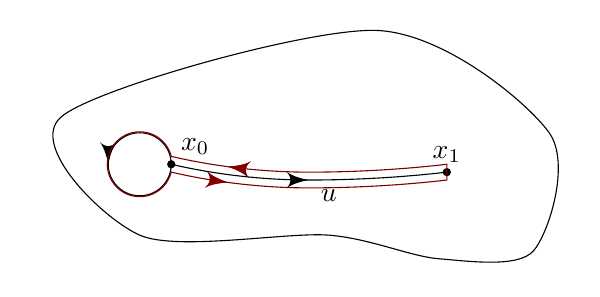
\begin{tikzpicture}
    \draw plot [smooth cycle] coordinates {(-2.4, -0.7) (0, -0.7) (1.4, -1) (2.6, -0.9) (2.8, 0.6) (0.6, 1.9) (-3.4, 0.8)};

    \node [circ] at (-2, 0.2) {};
    \node [anchor = south west] at (-2, 0.2) {$x_0$};
    \node [circ] at (1.5, 0.1) {};
    \node [above] at (1.5, 0.1) {$x_1$};

    \draw [->-=0.5] (-2.4, 0.2) circle [radius = 0.4];
    \draw [->-=0.5] (-2, 0.2) parabola bend (-0.25, 0) (1.5, 0.1) node [pos=0.5, below] {$u$};
    \draw [mred, ->-=0.3, ->-=0.7] (1.5, 0.1) -- (1.5, 0.2) parabola bend (-0.25, 0.1) (-2, 0.3) arc (14:346:0.4123) parabola bend (-0.25, -0.1) (1.5, 0) -- (1.5, 0.1);
  \end{tikzpicture}
\end{center}

\begin{prop}
  A path $u: x_0 \leadsto x_1$ induces a group \emph{isomorphism}
  \[
    u_\#: \pi_1(X, x_0) \to \pi_1(X, x_1)
  \]
  by
  \[
    [\gamma_0] \mapsto [u^{-1}\cdot \gamma \cdot u].
  \]
  This satisfies
  \begin{enumerate}
    \item If $u\simeq u'$, then $u_\# = u'_\#$.
    \item $(c_{x_0})_\# = \id_{\pi_1(X, x_0)}$
    \item If $v: x_1 \leadsto x_2$. Then $(u\cdot v)_\# = v_\# \circ u_\#$.
    \item If $f: X\to Y$ with $f(x_0) = y_0$, $f(x_1) = y_1$, then
      \[
        (f\circ u)_\# \circ f_* = f_* \circ u_\#: \pi_1(X, x_0) \to \pi_1(Y, y_1).
      \]
      A nicer way of writing this is
      \[
        \begin{tikzcd}[row sep=large]
          \pi_1(X, x_0) \ar[r, "f_*"] \ar[d, "u_\#"] & \pi_1(Y, y_0)\ar [d, "(f\circ u)_\#"]\\
          \pi_1(X, x_1) \ar[r, "f_*"] & \pi_1(Y, y_1)
        \end{tikzcd}
      \]
      The property says that the composition is the same no matter which way we go from $\pi_1(X, x_0)$ to $\pi_1(Y, y_1)$. We say that the square is a \emph{commutative diagram}. These diagrams will appear all of the time in this course.
    \item If $x_1 = x_0$, then $u_\#$ is an automorphism of $\pi_1(X, x_0)$ given by conjugation by $u$.
  \end{enumerate}
\end{prop}
It is important (yet difficult) the get the order of concatenation and composition right. Path concatenation is from left to right, while function composition is from right to left.

\begin{proof}
  Yet another exercise. Note that $(u^{-1})_\# = (u_\#)^{-1}$, which is why we have an isomorphism.
\end{proof}
The main takeaway is that if $x_0$ and $x_1$ are in the same path component, then
\[
  \pi_1(X, x_0) \cong \pi_1(X, x_1).
\]
So the basepoint isn't really too important. However, we have to be careful. While the two groups are isomorphic, the actual isomorphism depends on \emph{which} path $u: x_0 \leadsto x_1$ we pick. So there is no natural isomorphism between the two groups. In particular, we cannot say ``let $\alpha \in \pi_1(X, x_0)$. Now let $\alpha'$ be the corresponding element in $\pi_1(X, x_1)$''.

We can also see if $(X, x_0)$ and $(Y, y_0)$ are based homotopy equivalent, then $\pi_1(X, x_0)\cong \pi_1(Y, y_0)$. Indeed, if they are homotopy equivalent, then there is some $f: X \to Y$, $g: Y \to X$ such that $f\circ g = \id_Y$, $g\circ f = \id_X$. So $f_*\circ g_* = \id_{\pi_1(Y, y_0)}$ and $g_*\circ f_* = \id_{\pi_1(X, x_0)}$, and $f_*$ and $g_*$ are the isomorphisms we need.

However, can we do this with non-based homotopies? Suppose we have a space $X$, and a space $Y$, and functions $f, g: X \to Y$, with a homotopy $H: X\times I \to Y$ from $f$ to $g$. Since we don't insist that this fixes $x_0$, we could have $f(x_0) \not= g(x_0)$. What can we do?

First of all, we can find a path from $f(x_0)$ to $g(x_0)$. To produce this, we can use the homotopy. We let $u: f(x_0) \leadsto g(x_0)$ with $u = H(x_0, \cdot)$. Now we have things like $f_*, g_*$ and $u_\#$. Fortunately, these do fit together well.
\begin{center}
  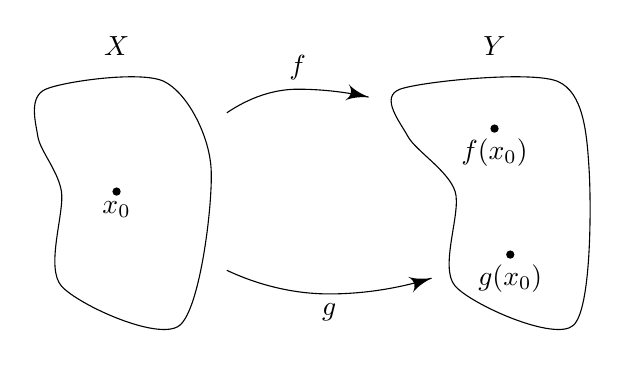
\begin{tikzpicture}
    \draw plot [smooth cycle] coordinates {(-3.7, -1.2) (-3.7, 0) (-4, 0.7) (-3.9, 1.3) (-2.4, 1.4) (-1.8, 0.3) (-2.2, -1.7)};
    \draw plot [smooth cycle] coordinates {(1.3, -1.2) (1.3, 0) (0.7, 0.7) (0.6, 1.3) (2.6, 1.4) (3, 0.3) (2.8, -1.7)};

    \node [circ] at (-3, 0) {};
    \node [below] at (-3, 0) {$x_0$};
    \node [above] at (-3, 1.6) {$X$};

    \node [above] at (1.8, 1.6) {$Y$};

    \node [circ] at (1.8, 0.8) {};
    \node [below] at (1.8, 0.8) {$f(x_0)$};

    \node [circ] at (2, -0.8) {};
    \node [below] at (2, -0.8) {$g(x_0)$};

    \draw [->] (-1.6, 1) parabola bend (-0.7, 1.3) (0.2, 1.2);
    \node [above] at (-0.7, 1.3) {$f$};

    \draw [->] (-1.6, -1) parabola bend (-0.3, -1.3) (1, -1.1);
    \node [below] at (-0.3, -1.3) {$g$};
  \end{tikzpicture}
\end{center}

\begin{lemma}
  The following diagram commutes:
  \[
    \begin{tikzcd}
      & \pi_1(Y, f(x_0)) \ar[dd, "u_\#"]\\
      \pi_1(X, x_0) \ar[ru, "f_*"] \ar [rd, "g_*"']& \\
      & \pi_1(Y, g(x_0))
    \end{tikzcd}
  \]
  In algebra, we say
  \[
    g_* = u_\# \circ f_*.
  \]
\end{lemma}

\begin{proof}
  Given a loop $\gamma: I\to X$ based at $x_0$.

  We need to check that
  \[
    g_*([\gamma]) = u_\#\circ f_*([\gamma]).
  \]
  In other words, we want to show that
  \[
    g\circ \gamma \simeq u^{-1}\cdot (f\circ \gamma)\cdot u.
  \]
  To prove this result, we want to build a homotopy.

  Consider the composition:
  \[
    F:
    \begin{tikzcd}
      I\times I \ar[r, "\gamma\times \id_I"] & X\times I \ar[r, "H"] & Y.
    \end{tikzcd}
  \]
  Our plan is to exhibit two homotopic paths $\ell^+$ and $\ell^-$ in $I\times I$ such that
  \[
    F\circ \ell^+ = g \circ \gamma,\quad F\circ \ell^- = u^{-1}\cdot (f\circ \gamma) \cdot u.
  \]
  This is in general a good strategy --- $X$ is a complicated and horrible space we don't understand. So to construct a homotopy, we make ourselves work in a much nicer space $I\times I$.

  Our $\ell^+$ and $\ell^-$ are defined in a rather simple way.
  \begin{center}
    \begin{tikzpicture}[scale=0.75]
      \node at (2, 5) {$I\times I$};
      \draw [mgreen, ->-=0.5] (0, 4) -- (0, 0);
      \draw [mgreen, ->-=0.5] (0, 0) -- (4, 0) node [pos=0.5, below] {$\ell^-$};
      \draw [mgreen, ->-=0.5] (4, 0) -- (4, 4);

      \draw [mred, ->-=0.5] (0, 4) -- (4, 4) node [pos=0.5, above] {$\ell^+$};

      \draw [->] (4.5, 2) -- (6.5, 2) node [pos=0.5, above] {$F$};
      \begin{scope}[shift={(7, 0)}]
      \node at (2, 5) {$Y$};
        \draw [->-=0.5] (0, 4) -- (0, 0) node [pos=0.5, right] {$u^{-1}$};
        \draw [->-=0.5] (0, 0) -- (4, 0) node [pos=0.5, below] {$f$};
        \draw [->-=0.5] (4, 0) -- (4, 4) node [pos=0.5, right] {$u$};

        \draw [->-=0.5] (0, 4) -- (4, 4) node [pos=0.5, above] {$g$};
      \end{scope}

    \end{tikzpicture}
  \end{center}
  More precisely, $\ell^+$ is the path $s\mapsto (s, 1)$, and $\ell^-$ is the concatenation of the paths $s\mapsto (0, 1- s)$, $s \mapsto (s, 0)$ and $s\mapsto (1, s)$.

  Note that $\ell^+$ and $\ell^-$ are homotopic as paths. If this is not obvious, we can manually check the homotopy
  \[
    L(s, t) = t\ell^+(s) + (1 - t)\ell^- (s).
  \]
  This works because $I\times I$ is convex. Hence $F\circ \ell^+\simeq_{F\circ L} F\circ \ell^-$ as paths.

  Now we check that the compositions $F\circ \ell^{\pm}$ are indeed what we want. We have
  \[
    F\circ \ell^+ (s) = H(\gamma(s), 1) = g\circ \gamma.
  \]
  Similarly, we can show that
  \[
    F\circ \ell^-(s) = u^{-1}\cdot (f\circ \gamma)\cdot u.
  \]
\end{proof}
It is worth looking at this proof hard and truly understand what is going on, since this is a really good example of how we can construct interesting homotopies.

With this lemma, we can show that fundamental groups really respect homotopies.

\begin{thm}
  If $f: X\to Y$ is a homotopy equivalence, and $x_0 \in X$, then the induced map
  \[
    f_*: \pi_1(X, x_0) \to \pi_1(Y, f(x_0).
  \]
  is an isomorphism.
\end{thm}
While this seems rather obvious, it is actually non-trivial if we want to do it from scratch. While we are given a homotopy equivalence, we are given no guarantee that the homotopy respects our basepoints. So this proof involves some real work.

\begin{proof}
  Let $g: Y\to X$ be a homotopy inverse. So $f\circ g\simeq_H \id_Y$ and $g\circ f\simeq_H' \id_X$.
  \begin{center}
    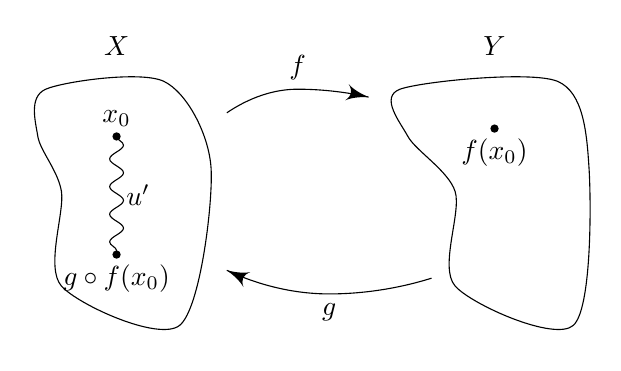
\begin{tikzpicture}
      \draw plot [smooth cycle] coordinates {(-3.7, -1.2) (-3.7, 0) (-4, 0.7) (-3.9, 1.3) (-2.4, 1.4) (-1.8, 0.3) (-2.2, -1.7)};
      \draw plot [smooth cycle] coordinates {(1.3, -1.2) (1.3, 0) (0.7, 0.7) (0.6, 1.3) (2.6, 1.4) (3, 0.3) (2.8, -1.7)};

      \node [circ] at (-3, 0.7) {};
      \node [above] at (-3, 0.7) {$x_0$};
      \node [above] at (-3, 1.6) {$X$};

      \node [above] at (1.8, 1.6) {$Y$};

      \node [circ] at (1.8, 0.8) {};
      \node [below] at (1.8, 0.8) {$f(x_0)$};

      \node [circ] at (-3, -0.8) {};
      \node [below] at (-3, -0.8) {$g\circ f(x_0)$};

      \draw [decoration={snake}, decorate] (-3, 0.7) -- (-3, -0.8) node [right, pos=0.5] {$u'$};

      \draw [->] (-1.6, 1) parabola bend (-0.7, 1.3) (0.2, 1.2);
      \node [above] at (-0.7, 1.3) {$f$};

      \draw [->] (1, -1.1) parabola bend (-0.3, -1.3) (-1.6, -1);
      \node [below] at (-0.3, -1.3) {$g$};
    \end{tikzpicture}
  \end{center}
  We have no guarantee that $g\circ f(x_0) = x_0$, but we know that our homotopy $H'$ gives us $u' = H'(x_0, \cdot): x_0 \leadsto g\circ f(x_0)$.

  Applying our previous lemma with $\id_X$ for ``$f$'' and $g \circ f$ for ``$g$'', we get
  \[
    u'_\# \circ (\id_X)_* = (g\circ f)_*
  \]
  Using the properties of the $_*$ operation, we get that
  \[
    g_*\circ f_* = u'_\#.
  \]
  However, we know that $u'_\#$ is an isomorphism. So $f_*$ is injective and $g_*$ is surjective.

  Doing it the other way round with $f\circ g$ instead of $g\circ f$, we know that $g_*$ is injective and $f_*$ is surjective. So both of them are isomorphisms.
\end{proof}
With this theorem, we can finally be sure that the fundamental group is a property of the space, without regards to the basepoint (assuming path connectedness), and is preserved by arbitrary homotopies.

We now use the fundamental group to define several simple notions.
\begin{defi}[Simply connected space]
  A space $X$ is \emph{simply connected} if it is path connected \emph{and} $\pi_1(X, x_0) \cong 1$ for some (any) choice of $x_0 \in X$.
\end{defi}

\begin{eg}
  Clearly, a point $*$ is simply connected since there is only one path on $*$ (the constant path). Hence, any contractible space is simply connected since it is homotopic to $*$. For example, $\R^n$ is simply connected for all spaces.
\end{eg}

There is a useful characterization of simply connected spaces:
\begin{lemma}
  A space $X$ is simply connected if and only if for any $x_0, x_1\in X$, there exists a unique homotopy class of paths $x_0 \leadsto x_1$.
\end{lemma}

Proof is, again, an exercise.

\section{Covering spaces}
We can ask ourselves a question --- what are groups? We can write down a definition in terms of operations and axioms, but this is not what groups \emph{are}. Groups were created to represent \emph{symmetries} of objects. In particular, a group should be \emph{acting} on something. If not, something wrong is probably going on.

We have created the fundamental group. So what do they act on? Can we find something on which these fundamental groups act on?

An answer to this would also be helpful in more practical terms. So far we have not exhibited a non-trivial fundamental group. This would be easy if we can make the group act on something --- if the group acts non-trivially on our thing, then clearly the group cannot be trivial.

These things we act on are \emph{covering spaces}.

\subsection{Covering space}
Intuitively, a \emph{covering space} of $X$ is a pair $(\tilde{X}, p: \tilde{X} \to X)$, such that if we take any $x_0 \in X$, there is some neighbourhood $U$ of $x$ such that the pre-image of the neighbourhood is ``many copies'' of $U$.
\begin{center}
  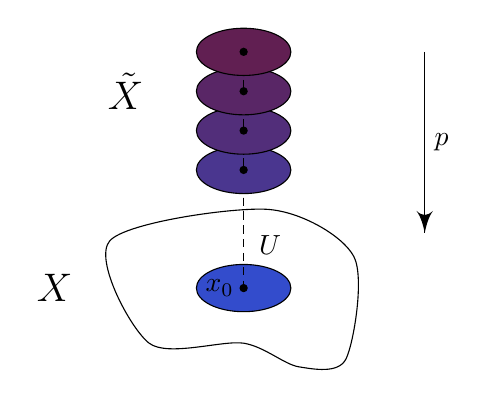
\begin{tikzpicture}
    \draw plot [smooth cycle] coordinates {(-1.2, -0.7) (0, -0.7) (0.7, -1) (1.3, -0.9) (1.4, 0.4) (0.3, 1) (-1.7, 0.6)};

    \draw [fill=mblue] ellipse (0.6 and 0.3);
    \node at (0.6, 0.3) [anchor = south east] {$U$};

    \draw [densely dashed] (0, 1.5) -- (0, 0);
    \foreach \y in {1.5, 2, 2.5, 3} {
      \node [circ] at (0, \y) {};
      \pgfmathsetmacro\c{100 - \y * 20};
      \draw [densely dashed] (0, \y) -- (0, \y - 0.5);
      \draw [fill=mblue!\c!mred] (0, \y) ellipse (0.6 and 0.3);
      \node [circ] at (0, \y) {};
    }
    \node at (-1.5, 2.5) {\Large $\tilde{X}$};
    \node at (-2.4, 0) {\Large $X$};
    \node [circ] at (0, 0) {};
    \node [left] at (0, 0) {$x_0$};

    \draw [->] (2.3, 3) -- (2.3, 0.7) node [right, pos=0.5] {$p$};
  \end{tikzpicture}
\end{center}

\begin{defi}[Covering space]
  A \emph{covering space} of $X$ is a pair $(\tilde{X}, p: \tilde{X} \to X)$, such that each $x\in X$ has a neighbourhood $U$ which is \emph{evenly covered}.
\end{defi}
Whether we require $p$ to be surjective is a matter of taste. However, it will not matter if $X$ is path-connected, which is the case we really care about.

\begin{defi}[Evenly covered]
  $U$ is \emph{evenly covered} by $p$ if
  \[
    p^{-1}(U) \cong \coprod_{\alpha \in \Lambda}V_\alpha,
  \]
  where $p|_{V_\alpha}: V_\alpha \to U$ is a homeomorphism, and each of the $V_\alpha$ is open.

  (the big reverse product sign is the disjoint union)
\end{defi}

\begin{eg}
  Homeomorphisms are covering maps. Duh.
\end{eg}

\begin{eg}
  Consider $p: \R \to S^1\subseteq \C$ defined by $t \mapsto e^{2\pi i t}$. This is a covering space.
  \begin{center}
    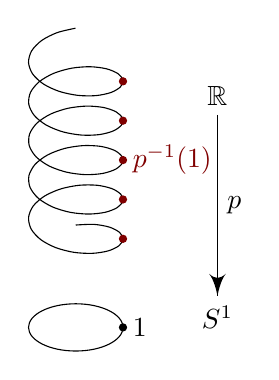
\begin{tikzpicture}
      \draw [samples=80, domain=0:5] plot [smooth] ({0.6 * sin (360 * \x)}, {1 + 0.3 * cos (360 * \x) + \x / 2});

      \draw ellipse (0.6 and 0.3);

      \node [circ] at (0.6, 0) {};
      \node [right] at (0.6, 0) {$1$};

      \foreach \y in {0,1,...,4} {
        \node [mred, circ] at (0.6, 1 + \y/2 + 0.125) {};
      }
      \node [mred, right] at (0.6, 2.125) {$p^{-1}(1)$};

      \draw [->] (1.8, 2.7) node [above] {$\R$}-- +(0, -2.3) node [pos=0.5, right] {$p$} node [below] {$S^1$};
    \end{tikzpicture}
  \end{center}
  Here we have $p^{-1}(1) = \Z$.
\end{eg}
As we said, we are going to use covering spaces to determine non-trivial fundamental groups. Before we do that, we can guess what the fundamental group of $S^1$ is. If we have a loop on $S^1$, it could be nothing, it can loop around the circle once, or loop around many times. So we can characterize each loop by the number of times it loops around the circle, and it should not be difficult to convince ourselves that two loops that loop around the same number of times can be continuously deformed to one another. So it is not unreasonable to guess that $\pi_1(S, 1) \cong \Z$. However, we also know that $p^{-1}(1) = \Z$. In fact, for any point $z\in S^1$, $p^{-1}(z)$ is just ``$\Z$ many copies'' of $z$. We will show that this is not a coincidence.

\begin{eg}
  Consider $p_n: S^1 \to S^1$ (for any $n \in \Z\setminus\{0\}$) defined by $z \mapsto z^n$.  We can consider this as ``winding'' the circle $n$ times, or as the following covering map:
  \begin{center}
    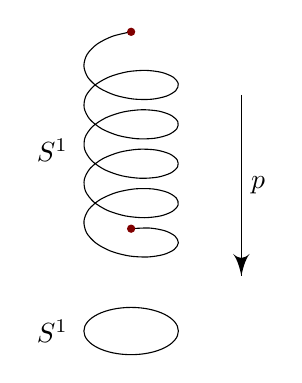
\begin{tikzpicture}
      \draw [samples=80, domain=0:5] plot [smooth] ({0.6 * sin (360 * \x)}, {1 + 0.3 * cos (360 * \x) + \x / 2});
      \node [circ, mred] at (0, 1.3) {};
      \node [circ, mred] at (0, 3.8) {};

      \draw ellipse (0.6 and 0.3);

      \node at (-1, 0) {$S^1$};
      \node at (-1, 2.3) {$S^1$};

      \draw [->] (1.4, 3) -- (1.4, 0.7) node [pos=0.5, right] {$p$};
    \end{tikzpicture}
  \end{center}
  where we join the two red dots together.

  This time the pre-image of $1$ would be $n$ copies of $1$, instead of $\Z$ copies of $1$.
\end{eg}

\begin{eg}
  Consider $X = \RP^2$, which is the real projective plane. This is defined by $S^2/{\sim}$, where we identify every $x\simeq -x$, ie. every pair of antipodal point. We can also think of this as the space of lines in $\R^3$.  This is actually really difficult to draw (and in fact impossible to fully embed in $\R^3$), so we will not attempt. There is, however, a more convenient way of thinking about $\RP^2$. We just use the definition --- we imagine an $S^2$, but this time, instead of a point being a ``point'' on the sphere, it is a \emph{pair} of antipodal points.
  \begin{center}
    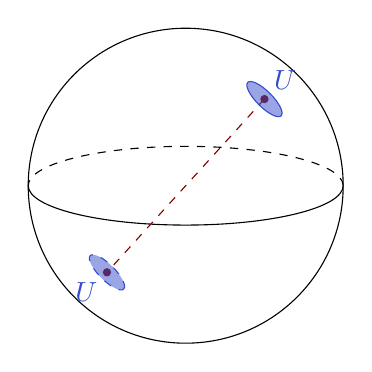
\begin{tikzpicture}
      \draw circle [radius=2];

      \draw [dashed] (2, 0) arc (0:180:2 and 0.5);
      \draw (-2, 0) arc (180:360:2 and 0.5);

      \draw [dashed, mred] (1, 1.1) node [circ] {} -- (-1, -1.1) node [circ] {};

      \draw [rotate around={-45:(1, 1.1)}, mblue, fill=mblue, fill opacity=0.5] (1, 1.1) ellipse (0.3 and 0.1) node [opacity=1, anchor = south west] {$U$};

      \draw [dashed, rotate around={-45:(-1, -1.1)}, mblue, fill=mblue, fill opacity=0.5] (-1, -1.1) ellipse (0.3 and 0.1) node [opacity=1, anchor = north east] {$U$};
    \end{tikzpicture}
  \end{center}
  We define $p: S^2 \to \RP^2$ to be the quotient map. Then this is a covering map, since the pre-image of a small neighbourhood of any $x_0$ is just two copies of the neighbourhood.
\end{eg}

\begin{defi}[Lifting]
  Let $f: Y\to X$ be a map, and $p: \tilde{X} \to X$ a covering space. A \emph{lift} of $f$ is a map $\tilde{f}: Y\to \tilde{X}$ such that $f = p\circ \tilde{f}$, ie. the following diagram commutes:
  \[
    \begin{tikzcd}
      & \tilde{X} \ar[d, "p"]\\
      Y \ar[ur, "\tilde{f}"] \ar [r, "f"] & X
    \end{tikzcd}
  \]
\end{defi}
Intuitively, instead of mapping to $X$, we map to one of the ``copies'' of $X$ in the covering space $\tilde{X}$.

We can visualize this in the case where $Y$ is the unit interval $I$ and the map is just a path in $X$.
\begin{center}
  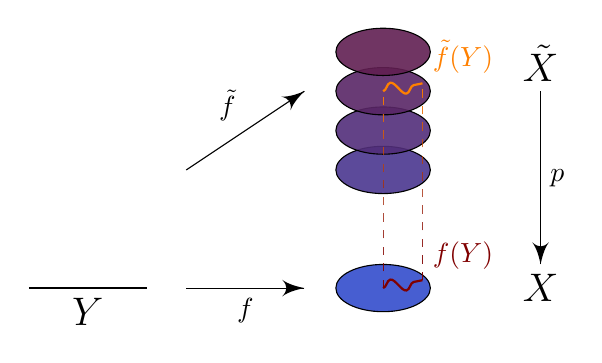
\begin{tikzpicture}
    \draw [fill=mblue, fill opacity=0.9] ellipse (0.6 and 0.3);

    \foreach \y in {1.5, 2, 2.5, 3} {
      \pgfmathsetmacro\c{100 - \y * 20};
      \draw [fill=mblue!\c!mred, fill opacity=0.9] (0, \y) ellipse (0.6 and 0.3);
    }

    \draw [->] (2, 2.5) node [above] {\Large $\tilde{X}$} -- +(0, -2.2) node [below] {\Large $X$} node [pos=0.5, right] {$p$};

    \draw [thick] (-4.5, 0) -- (-3, 0) node [pos=0.5, below] {\Large $Y$};

    \draw [->] (-2.5, 0) -- (-1, 0) node [below, pos=0.5] {$f$} ;
    \draw [->] (-2.5, 1.5) -- (-1, 2.5) node [anchor = south east, pos=0.5] {$\tilde{f}$};

    \draw [thick, mred, decoration={snake}, decorate] (0, 0) -- +(0.5, 0.1) node [anchor = south west] {$f(Y)$};
    \draw [thick, morange, decoration={snake}, decorate] (0, 2.5) -- +(0.5, 0.1) node [anchor = south west] {$\tilde{f}(Y)$};

    \draw [morange, dashed, path fading=south] (0, 0) -- +(0, 2.5);
    \draw [mred, dashed, path fading=north] (0, 0) -- +(0, 2.5);
    \draw [morange, dashed, path fading=south] (0.5, 0.1) -- +(0, 2.5);
    \draw [mred, dashed, path fading=north] (0.5, 0.1) -- +(0, 2.5);

  \end{tikzpicture}
\end{center}
It feels that if we know which ``copy'' of $X$ we lifted our map to, then we already know everything about $\tilde{f}$, since we are just moving our $f$ from $X$ to that particular copy of $X$. This is made precise by the following lemma:

\begin{lemma}
  Let $p: \tilde{X} \to X$ be a covering map, $f: Y\to X$ be a map, and $\tilde{f}_1 ,\tilde{f}_2$ are both lists of $f$. Then
  \[
    S = \{y\in Y: \tilde{f}_1(y) = \tilde{f}_2(y)\}
  \]
  is both open and closed. In particular, if $Y$ is connected, $\tilde{f}_1$ and $\tilde{f}_2$ agree either everywhere or nowhere.
\end{lemma}
This is sort of a ``uniqueness statement'' for a lift. If we know a point in the lift, then we know the whole path. This is since once we've decided our starting point, ie, which ``copy'' of $X$ we work in, the rest of $\tilde{f}$ has follow what $f$ does.

\begin{proof}
  Exercise. % fill in.
\end{proof}

We just had a uniqueness statement. Given a map, is the guarantee that we can lift it to something? In particular, if I have fixed a ``copy'' of $X$ I like, can I also lift my map to that copy? This is given by the following lemma:

\begin{lemma}[Homotopy lifting lemma]
  Let $p: \tilde{X} \to X$ be a covering space, $H: Y\times I \to X$ be a homotopy from $f_0$ to $f_1$. Let $\tilde{f}_0$ be a lift of $f_0$. Then there exists a \emph{unique} homotopy $\tilde{H}: Y\times I \to \tilde{X}$ such that
  \begin{enumerate}
    \item $\tilde{H}(\cdot, 0) = \tilde{f}_0$; and
    \item $\tilde{H}$ is a lift of $H$, ie. $p\circ\tilde{H} = H$.
  \end{enumerate}
\end{lemma}
This lemma might be difficult to comprehend at first. We can look at the special case where $Y = *$. Then a homotopy is just a path. So the lemma specializes to
\begin{lemma}[Path lifting lemma]
  Let $p: \tilde{X} \to X$ be a covering space, $\gamma: I\to X$ a path, and $\tilde{x}_0 \in \tilde{X}$ such that $p(\tilde{x}_0) = x_0 = \gamma(0)$. Then there exists a \emph{unique} path $\tilde{\gamma}: I\to \tilde{X}$ such that
  \begin{enumerate}
    \item $\tilde{\gamma}(0) = \tilde{x}_0$; and
    \item $\tilde{\gamma}$ is a lift of $\gamma$, ie. $p\circ \tilde{\gamma} = \gamma$.
  \end{enumerate}
\end{lemma}
This is exactly the picture we were drawing before. We just have to start at a point $\tilde{x}_0$, and then everything is determined because locally, everything upstairs in $\tilde{X}$ is just like $X$. Note that we have already proved uniqueness. So we just need to prove existence.

In theory, it makes sense to prove homotopy lifting, and path lifting comes immediately as a corollary. However, the proof of homotopy lifting is big and scary. So instead, we will prove path lifting, which is something we can more easily visualize and understand, and then use that to prove homotopy lifting.

\begin{proof}(sketch proof of path lifting)
  Let
  \[
    S = \{s \in I: \tilde{\gamma}\text{ exists on }[0, s] \subseteq I\}.
  \]
  Observe that
  \begin{enumerate}
    \item $0\in S$
    \item $S$ is closed. It is obvious that if $s \in S$, then any $t < s$ would be in $S$ as well. Also, if $s_n \to s_{\infty}$, we can set $\tilde{\gamma}(s) = \lim_{n \to \infty}\tilde{\gamma}(s_n)$, then everything works. So $\tilde{\gamma}$ is defined at $s_{\infty}$. Note that here uniqueness helps a lot, since this tells us that $\tilde{\gamma}(s_n)$ is well-defined.

    \item $S$ is open. If $s\in S$ and $\tilde{\gamma}(s) \in V_\beta \subseteq p^{-1}(U)$, we can define $\tilde{\gamma}$ on some small neighbourhood of $s$ by
      \[
        \tilde{\gamma}(t) = (p|_{V_\beta})^{-1}\circ \gamma
      \]
  \end{enumerate}
  Since $S$ is both open and closed, we have $S = I$. So $\tilde{\gamma}$  exists.
\end{proof}
How can we promote this to a proof of the homotopy lifting lemma? At every point $y\in Y$, we know what to do, since we have path lifting. So $\tilde{H}(y, \cdot)$ is defined. So the thing we have to do is to show that this is continuous. Steps of the proof are
\begin{enumerate}
  \item Use compactness of $I$ to argue that the proof of path lifting works on small neighbourhoods in $Y$.
  \item For each $y$, we pick an open neighbourhood $U$ of $y$, and define a good path lifting on $U\times I$.
  \item By uniqueness of liftings, these path liftings agree when they overlap. So we have one big continuous lifting.
\end{enumerate}
% could expand a bit

With th homotopy lifting lemma in our toolkit, we can start to use it to do stuff. So far, we have covering spaces and fundamental groups. We are now going to build a bridge between these two, and show how covering spaces can be used to reflect some structures of the fundamental group.

At least one payoff of this work is that we are going to exhibit some non-trivial fundamental groups.

We have just showed that we are allowed to lift homotopies. However, what we are really interested in is homotopy \emph{as paths}. The homotopy lifting lemma does not tell us that the lifted homotopy preserves basepoints. This is what we are going to show.

\begin{cor}
  Suppose $\gamma, \gamma': I\to X$ are paths $x_0 \leadsto x_1$ and $\tilde{g}, \tilde{g}': I\to \tilde{X}$ are lifts of $\gamma$ and $\gamma'$ respectively, both starting at $\tilde{x}_0 \in p^{-1}(x_0)$.

  If $\gamma\simeq \gamma'$ as \emph{paths}, then $\tilde{\gamma}$ and $\tilde{\gamma}'$ are homotopic as paths. In particular, $\tilde{\gamma}(1) = \tilde{\gamma}'(1)$.
\end{cor}
Note that if we cover the words ``as paths'' and just talk about homotopies, then this is just the homotopy lifting lemma. So we can view this as a stronger form of the homotopy lifting lemma.

\begin{proof}
  The homotopy lifting lemma gives as a $\tilde{H}$, a lift of $H$ with $\tilde{H}(\cdot, 0) = \tilde{\gamma}$.
  \begin{center}
    \begin{tikzpicture}
      \begin{scope}
        \draw (0, 0) rectangle (2, 2);
        \node at (1, 0) [below] {$\gamma$};
        \node at (1, 2) [above] {$\gamma'$};
        \node at (0, 1) [left] {$c_{x_0}$};
        \node at (2, 1) [right] {$c_{x_1}$};
        \node at (1, 1) {\Large $H$};
      \end{scope}

      \draw [->] (3, 1) -- (5, 1) node [pos=0.5, above] {lift};
      \begin{scope}[shift={(6, 0)}]
        \draw (0, 0) rectangle (2, 2);
        \node at (1, 0) [below] {$\tilde{\gamma}$};
        \node [gray] at (1, 2) [above] {$\tilde{\gamma'}$};
        \node [gray] at (0, 1) [left] {$c_{\tilde{x}_0}$};
        \node [gray] at (2, 1) [right] {$c_{\tilde{x}_1}$};
        \node at (1, 1) {\Large $\tilde{H}$};
      \end{scope}
    \end{tikzpicture}
  \end{center}
  In this diagram, we have showed that the bottom of the $\tilde{H}$ square is $\tilde{\gamma}$. To show that this is a path homotopy from $\tilde{\gamma}$ to $\tilde{\gamma'}$, we need to show that the other edges are $c_{\tilde{x}_0}$, $c_{\tilde{x}_1}$ and $\tilde{\gamma}'$ respectively.


  Now $\tilde{H}(\cdot, 1)$ is a lift of $H(\cdot, 1) = \gamma'$, starting at $\tilde{x}_0$. Since lifts are unique, we must have $\tilde{H}(\cdot, 1) = \tilde{\gamma}'$. So this is indeed a homotopy between $\tilde{\gamma}$ and $\tilde{\gamma}'$. Now we need to check that this is a homotopy of paths.

  We know that $\tilde{H}(0, \cdot)$ is a lift of $H(0, \cdot) = c_{x_0}$. We are aware of one lift of $c_{x_0}$, namely $c_{\tilde{x}_0}$. By uniqueness of lift, we must have $\tilde{H}(0, \cdot) = c_{\tilde{x}_0}$. Similarly, $\tilde{H}(1, \cdot) = c_{\tilde{x}_1}$. So this is a homotopy of paths.
\end{proof}

So far, our picture of covering spaces is like this:
\begin{center}
  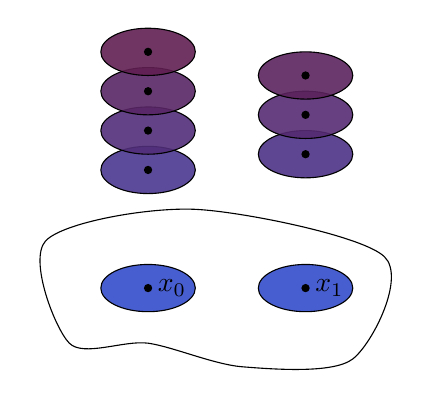
\begin{tikzpicture}
    \draw plot [smooth cycle] coordinates {(-1, -0.7) (0, -0.7) (1.2, -1) (2.6, -0.9) (3, 0.4) (0.6, 1) (-1.3, 0.6)};

    \draw [fill=mblue, fill opacity=0.9] ellipse (0.6 and 0.3);
    \node [circ] at (0, 0) {};
    \node [right] at (0, 0) {$x_0$};
    \foreach \y in {1.5, 2, 2.5, 3} {
      \pgfmathsetmacro\c{100 - \y * 20};
      \draw [fill=mblue!\c!mred, fill opacity=0.9] (0, \y) ellipse (0.6 and 0.3);
      \node [circ] at (0, \y) {};
    }

    \begin{scope}[shift={(2, 0)}]
      \draw [fill=mblue, fill opacity=0.9] ellipse (0.6 and 0.3);
      \node [circ] at (0, 0) {};
      \node [right] at (0, 0) {$x_1$};
      \foreach \y in {1.7, 2.2, 2.7} {
        \pgfmathsetmacro\c{100 - \y * 20};
        \draw [fill=mblue!\c!mred, fill opacity=0.9] (0, \y) ellipse (0.6 and 0.3);
        \node [circ] at (0, \y) {};
      }
    \end{scope}
  \end{tikzpicture}
\end{center}
Except\ldots is it? Is it possible that we have four copies of $x_0$ but just three copies of $x_1$? This is obviously possible if $X$ is not path connected --- the component containing $x_0$ and the one containing $x_1$ are completely unrelated. But what if $X$ is path connected?

\begin{cor}
  If $X$ is a path connected space, $x_0, x_1 \in X$, then there is a bijection $p^{-1}(x_0) \to p^{-1}(x_1)$.
\end{cor}

\begin{proof}
  Let $\gamma: x_0 \leadsto x_1$ be a path. We want to use this to construct a bijection between each preimage of $x_0$ and each preimage of $x_1$. The obvious thing to use is to use lifts of the path $\gamma$.
  \begin{center}
    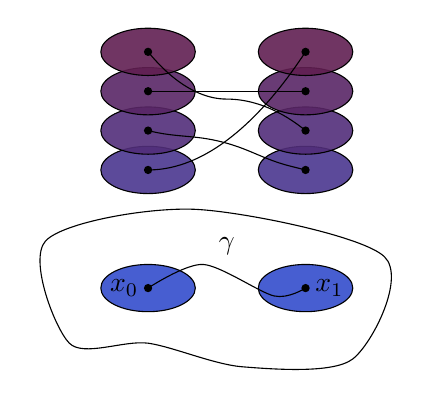
\begin{tikzpicture}
      \draw plot [smooth cycle] coordinates {(-1, -0.7) (0, -0.7) (1.2, -1) (2.6, -0.9) (3, 0.4) (0.6, 1) (-1.3, 0.6)};

      \draw [fill=mblue, fill opacity=0.9] ellipse (0.6 and 0.3);
      \node [circ] at (0, 0) {};
      \node [left] at (0, 0) {$x_0$};
      \foreach \y in {1.5, 2, 2.5, 3} {
        \pgfmathsetmacro\c{100 - \y * 20};
        \draw [fill=mblue!\c!mred, fill opacity=0.9] (0, \y) ellipse (0.6 and 0.3);
        \node [circ] at (0, \y) {};
      }

      \begin{scope}[shift={(2, 0)}]
        \draw [fill=mblue, fill opacity=0.9] ellipse (0.6 and 0.3);
        \node [circ] at (0, 0) {};
        \node [right] at (0, 0) {$x_1$};
        \foreach \y in {1.5, 2, 2.5, 3} {
          \pgfmathsetmacro\c{100 - \y * 20};
          \draw [fill=mblue!\c!mred, fill opacity=0.9] (0, \y) ellipse (0.6 and 0.3);
          \node [circ] at (0, \y) {};
        }
      \end{scope}

      \draw plot [smooth] coordinates {(0, 0) (0.7, 0.3) (1.6, -0.1) (2, 0)};
      \node at (1, 0.3) [above] {$\gamma$};

      \draw (0, 1.5) parabola (2, 3);
      \draw [decorate, decoration={snake, segment length=3cm}] (0, 2) -- (2, 1.5);
      \draw (0, 3) parabola bend (1, 2.4) (2, 2);
      \draw (0, 2.5) -- (2, 2.5);
    \end{tikzpicture}
  \end{center}
  Define a map $p^{-1}(x_0) \to p^{-1}(x_1)$ that sends $\tilde{x}_0$ to the end point of the unique lift of $\gamma$ at $\tilde{x}_0$.

  The inverse map is obtained by replacing $\gamma$ with $\gamma^{-1}$. It is an exercise to show that this is indeed an inverse.
  % complete
\end{proof}

\begin{defi}[$n$-sheeted]
  A covering space $p: \tilde{X} \to X$ of a path-connected space $X$ is $n$-\emph{sheeted} if $|p^{-1}(x)| = n$ for all $x \in X$.
\end{defi}
Each covering space has a number associated to it, namely the number of sheets. Is there any number we can assign to fundamental groups? Well, the index of a subgroup might be a good candidate. We'll later see if this is the case.

\begin{lemma}
  If $p: \tilde{X} \to X$ is a covering map and $\tilde{x}_0 \in \tilde{X}$, then
  \[
    p_*: \pi_1(\tilde{X}, \tilde{x}_0) \to \pi_1(X, x_0)
  \]
  is injective.
\end{lemma}

\begin{proof}
  To show that at a group homomorphism $p_*$ is injective, we have to show that if $p_*(x)$ is trivial, then $x$ must be trivial.

  Consider a based loop $\tilde{\gamma}$ in $\tilde{X}$. We let $\gamma = p\circ \tilde{\gamma}$. If $\gamma$ is trivial, ie. $\gamma \simeq c_{x_0}$ as paths, The homotopy lifting lemma them gives us a homotopy upstairs between $\tilde{\gamma}$ and $c_{\tilde{x}_0}$. So $\tilde{\gamma}$ is trivial.
\end{proof}

As we have originally said, our objective is to make our fundamental group act on something. We are almost there already.

Let's look again at the proof that there is a bijection between $p^{-1}(x_0)$ and $p^{-1}(x_1)$. What happens if $\gamma$ is a loop? For any $\tilde{x}_0 \in p^{-1}(x_0)$, we can look at the end point of the lift. This end point may or may not be our original $\tilde{x}_0$. So each loop $\gamma$ ``moves'' our $\tilde{x}_0$ to another $\tilde{x}_0'$.

However, we are not really interested in paths themselves. We are interested in equivalence classes of paths under homotopy of paths. However, this is fine. If $\gamma$ is homotopic to $\gamma'$, then this homotopy can be lifted to get a homotopy between $\tilde{\gamma}$ and $\tilde{\gamma}'$. In particular, these have the same end points. So each (based) homotopy class gives a well-defined endpoint.
\begin{center}
  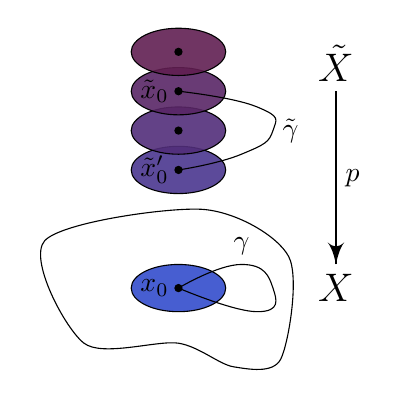
\begin{tikzpicture}
    \draw plot [smooth cycle] coordinates {(-1.2, -0.7) (0, -0.7) (0.7, -1) (1.3, -0.9) (1.4, 0.4) (0.3, 1) (-1.7, 0.6)};
    \draw [fill=mblue, fill opacity=0.9] ellipse (0.6 and 0.3);

    \foreach \y in {1.5, 2, 2.5, 3} {
      \pgfmathsetmacro\c{100 - \y * 20};
      \draw [fill=mblue!\c!mred, fill opacity=0.9] (0, \y) ellipse (0.6 and 0.3);
      \node [circ] at (0, \y) {};
    }

    \draw [->] (2, 2.5) node [above] {\Large $\tilde{X}$} -- +(0, -2.2) node [below] {\Large $X$} node [pos=0.5, right] {$p$};

    \node [circ] at (0, 0) {};
    \node [left] at (0, 0) {$x_0$};

    \draw plot [tension=0.9, smooth] coordinates {(0, 0) (1, -0.3) (1.2, 0) (0.8, 0.3) (0, 0)};
    \node at (0.8, 0.3) [above] {$\gamma$};

    \draw plot [tension=0.9, smooth] coordinates {(0, 2.5) (1, 2.3) (1.2, 2) (0.8, 1.7) (0, 1.5)};
    \node [right] at (1.2, 2) {$\tilde{\gamma}$};

    \node [left] at (0, 2.5) {$\tilde{x}_0$};
    \node [left] at (0, 1.5) {$\tilde{x}_0'$};
  \end{tikzpicture}
\end{center}
Now this gives an action of $\pi_1(X, x_0)$ on $p^{-1}(x_0)$! Note, however, that this will not be the sort of actions we are familiar with. We usually work with \emph{left}-actions, where the group acts on the left, but now we will have \emph{right}-actions, which may confuse you a lot. To see this, we have to consider what happens when we perform two operations one after another. We write this action as $\tilde{x}_0 \cdot [\gamma]$.

When we have an action, we are interested in two things --- the orbits, and the stabilizers. This is what the next lemma tells us about.

\begin{lemma}
  Suppose $X$ is path connected and $x_0 \in X$.
  \begin{enumerate}
    \item The action of $\pi_1(X, x_0)$ on $p^{-1}(x_0)$ is transitive if and only if $\tilde{X}$ is path connected. Alternatively, we can say that the orbits ofthe action correspond to the path components.
    \item The stabilizer of $\tilde{x}_0 \in p^{-1}(x_0)$ is $p_*(\pi(\tilde{X}, \tilde{x}_0)) \subseteq \pi(X, x_0)$.
    \item If $\tilde{X}$ is path connected, then there is a bijection
      \[
        p_* \pi_1(\tilde{X}, \tilde{x}_0)\backslash p_* \pi_1(\tilde{X}\tilde{x}_0) \to p^{-1}(x_0).
      \]
      Note that $p_* \pi_1(\tilde{X}, \tilde{x}_0)\backslash p_* \pi_1(\tilde{X}\tilde{x}_0)$ is not a quotient, but simply the set of cosets. We write it the ``wrong way round'' because we have right cosets instead of left cosets.
  \end{enumerate}
\end{lemma}
Note that this is great! If we can find a covering space $p$ and a point $x_0$ such that $p^{-1}(x_0)$ is non-trivial, then we immediately know that $\pi_1(X, x_0)$ is non-trivial!

\begin{proof}\leavevmode
  \begin{enumerate}
    \item If $\tilde{x}_0, \tilde{x}'_0 \in p^{-1}(x_0)$, then since $\tilde{X}$ is path connected, we know that there is some $\tilde{\gamma}: \tilde{x}_0 \leadsto \tilde{x}_0'$. Then we can project this to $\gamma = p\circ \tilde{\gamma}$. Then $\gamma$ is a path from $x_0 \leadsto x_0$, ie. a loop. Then by the definition on the action, $\tilde{x}_0 \cdot [\gamma] = \tilde{\gamma}(1) = \tilde{x}_0'$.

    \item Suppose $[\gamma] \in \stab(\tilde{x}_0)$. Then $\tilde{\gamma}$ is a loop based at $\tilde{x_0}$. So $\tilde{\gamma}$ defines $[\tilde{\gamma}] \in \pi_1(\tilde{X}, \tilde{x}_0)$ and $\gamma = p\circ \tilde{\gamma}$.

    \item This follows directly from the orbit-stabilizer theorem.
  \end{enumerate}
\end{proof}

We now want to use this to determine that the fundamental group of a space is non-trivial. We can be more ambitious, and try to actually \emph{find} $\pi_1(X, x_0)$. In the best possible scenario, we would have $\pi_1(\tilde{X}, \tilde{x}_0)$ trivial. Then we have a bijection between $\pi_1(X, x_0)$ and $p^{-1}(x_0)$. In other words, we want our covering space $\tilde{X}$ to be simply connected.

\begin{defi}[Universal cover]
  A covering map $p: \tilde{X} \to X$ is a \emph{universal cover} if $\tilde{X}$ is simply connected.
\end{defi}

\begin{cor}
  If $p: \tilde{X} \to X$ is a universal cover, then there is a bijection $\ell: \pi_1(X, x_0) \to p^{-1}(x_0)$.
\end{cor}
Note that the orbit stabilizer theorem does not provide a canonical bijection between $p^{-1}(x_0)$ and $p_* \pi_1(\tilde{X}, \tilde{x}_0)\backslash p_* \pi_1(\tilde{X}\tilde{x}_0)$. To obtain a bijection, we need to pick a starting point $\tilde{x}_0 \in p^{-1}(x_0)$. So the above bijection $\ell$ depends on a choice of $\tilde{x}_0$.

\subsection{The fundamental group of the circle and its applications}
Finally, we can exhibit a non-trivial fundamental group. We are going to consider the space $S^1$ and a universal covering $\R$.
\begin{center}
  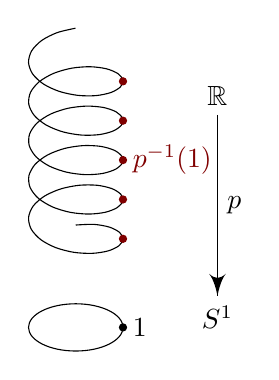
\begin{tikzpicture}
    \draw [samples=80, domain=0:5] plot [smooth] ({0.6 * sin (360 * \x)}, {1 + 0.3 * cos (360 * \x) + \x / 2});

    \draw ellipse (0.6 and 0.3);

    \node [circ] at (0.6, 0) {};
    \node [right] at (0.6, 0) {$1$};

    \foreach \y in {0,1,...,4} {
      \node [mred, circ] at (0.6, 1 + \y/2 + 0.125) {};
    }
    \node [mred, right] at (0.6, 2.125) {$p^{-1}(1)$};

    \draw [->] (1.8, 2.7) node [above] {$\R$} -- +(0, -2.3) node [pos=0.5, right] {$p$} node [below] {$S^1$};
  \end{tikzpicture}
\end{center}
Then our previous corollary gives
\begin{cor}
  There is a bijection $\pi_1(S^1, 1) \to p^{-1}(1) = \Z$.
\end{cor}
What's next? We just know that $\pi_1(S^1, 1)$ is countably infinite, but can we work out the group structure?

We can, in fact, prove a stronger statement:
\begin{thm}[]
  The map $\ell: \pi_1(S^1, 1) \to p^{-1}(1) = \Z$ is a group isomorphism.
\end{thm}

\begin{proof}
  We know it is a bijection. So we need to check it is a group homomorphism. The idea is to write down representatives for what we think the elements should be.
  \begin{center}
    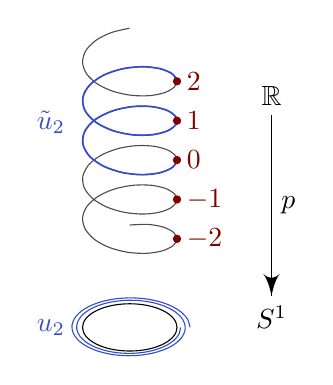
\begin{tikzpicture}
      \draw [samples=80, domain=0:5, opacity=0.7] plot [smooth] ({0.6 * sin (360 * \x)}, {1 + 0.3 * cos (360 * \x) + \x / 2});

      \draw [mblue, semithick, domain=2.25:4.25, samples=30] plot [smooth] ({0.6 * sin (360 * \x)}, {1 + 0.3 * cos (360 * \x) + \x / 2});

      \node [mblue] at (-1, 2.6) {$\tilde{u}_2$};
      \foreach \y in {-2,-1,...,2} {
        \node [mred, circ] at (0.6, 2 + \y/2 + 0.125) {};
        \node [mred, right] at (0.6, 2 + \y/2 + 0.125) {$\y$};
      }

      \draw ellipse (0.6 and 0.3);

      \draw [->] (1.8, 2.7) node [above] {$\R$} -- +(0, -2.3) node [pos=0.5, right] {$p$} node [below] {$S^1$};

      \draw [domain=0.25:2.25, mblue, samples=50] plot [smooth] ({(1.05 + \x / 10) *  0.6 * sin (360 * \x)}, {(1.05 + \x / 10) * 0.3 * cos (360 * \x)});
      \node [mblue] at (-1, 0) {$u_2$};
    \end{tikzpicture}
  \end{center}
  Let $\tilde{u}_n: I \to \R$ be defined by $t \mapsto nt$, and let $u_n = p\circ \tilde{u}_n$. Note that for any $[\gamma] \in \pi_1(S^1, 1)$, if $\tilde{\gamma}$ is a lift to $\R$ at $0$ and $\tilde{\gamma}(1) = n$, then $\tilde{\gamma} \simeq \tilde{u_n}$ as paths (because $\R$ is simply connected, so there is a unique homotopy class between any two points). So $[\gamma] = [u_n]$.

  To show that this has the right group operation, we can easily that $\widetilde{u_m \cdot u_n} = \tilde{u}_{m + n}$, since we are just moving by $n + m$ in both cases. Therefore
  \[
    \ell([u_m][u_n]) = \ell([u_m \cdot u_m]) = m + n = \ell([u_{m + n}]).
  \]
  So $\ell$ is a homotopy equivalence.
\end{proof}
What have we done? In general, we might be given a horrible, crazy loop in $S^1$. It would be rather difficult to work with it directly in $S^1$. So we pull it up to the universal covering $\R$. Since $\R$ is nice and simply connected, we can easily produce a homotopy that ``straightens out'' the path. We then project this homotopy down to $S^1$, to get a homotopy from $\gamma$ to $u_n$.

It is indeed possible to produce a homotopy directly inside $S^1$ from each loop to some $u_n$, but that would be tedious work that involves messing with a lot of algebra and weird, convoluted formulas.

From the fundamental group of the circle, we can deduce many things. An immediate application is that we can properly define the ``winding number'' of a function. Also, we have the following classic application:
\begin{thm}[Brouwer's fixed point theorem]
  Let $D^2 = \{(x, y) \in \R^2: x^2 + y^2 = 1\}$ by the unit disk. If $f: D^2 \to D^2$ is continuous, then there is some $x\in D^2$ such that $f(x) = x$.
\end{thm}

\begin{proof}
  Suppose not. So $x \not= f(x)$ for all $x\in D^2$.
  \begin{center}
    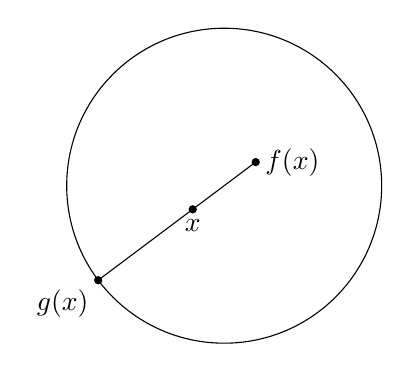
\begin{tikzpicture}
      \draw circle [radius=2cm];
      \node [circ] at (-0.4, -0.3) {};
      \node at (-0.4, -0.3) [below] {$x$};

      \node [circ] at (0.4, 0.3) {};
      \node at (0.4, 0.3) [right] {$f(x)$};
      \draw (0.4, 0.3) -- (-1.6, -1.2);
      \node at (-1.6, -1.2) [circ] {};
      \node at (-1.6, -1.2) [anchor = north east] {$g(x)$};
    \end{tikzpicture}
  \end{center}
  We define $g: D^2 \to S^1$ as in the picture above. Then we know that $g$ is continuous and $g$ is a \emph{retraction} from $D^2$ onto $S^1$. In other words, the following composition is the identity:
  \[
    \begin{tikzcd}
      S^1 \ar[r, hook, "\iota"] \ar[rr, bend right, "\id_{S^1}"'] & D^2 \ar[r, "g"] & S^1
    \end{tikzcd}
  \]
  Then this induces a homomorphism of groups whose composition is the identity:
  \[
    \begin{tikzcd}
      \Z \ar[r, hook, "\iota_*"] \ar[rr, bend right, "\id_\Z"'] & \{0\} \ar[r, "g_*"] & \Z
    \end{tikzcd}
  \]
  But this is clearly nonsense! So we must have had a fixed point.
\end{proof}
But we have a problem. What about $D^3$? Can we prove a similar theorem? Here the fundamental group is of little use, since we can show that the fundamental group of $S^n$ for $n \geq 2$ is trivial. Later in the course, we will be able to prove this theorem for higher dimensions, when we have developed more tools to deal with stuff.

\subsection{Universal covers}
We have defined universal covers mysteriously as covers that are simply connected. We have just shown that $p: \R\to S^1$ is a universal cover. In general, what do universal covers look like?

Let's consider a slightly more complicated example. What would be a universal cover of the torus $S^1 \times S^1$? An obvious guess would be $p\times p: \R\times \R \to S^1 \times S^1$. How can we visualize this?

First of all, how can we visualize a torus? Often, we just picture it as the surface of a doughnut. Alternatively, we can see it as a quotient of the square, where we identify the following edges:
\begin{center}
  \begin{tikzpicture}
    \draw [->-=0.55, mred] (0, 0) -- (3, 0);
    \draw [->-=0.55, mred] (0, 3) -- (3, 3);

    \draw [->-=0.55, mblue] (0, 0) -- (0, 3);
    \draw [->-=0.55, mblue] (3, 0) -- (3, 3);
  \end{tikzpicture}
\end{center}
Then what does it \emph{feel} like to live in the torus? If you live in a torus and look around, you wouldn't see a boundary. The space just extends indefinitely for ever, somewhat like $\R^2$. The difference is that in the torus, you aren't actually seeing free space out there, but just seeing copies of the same space over and over again. If you live inside the square, the universe actually looks like this:
\begin{center}
  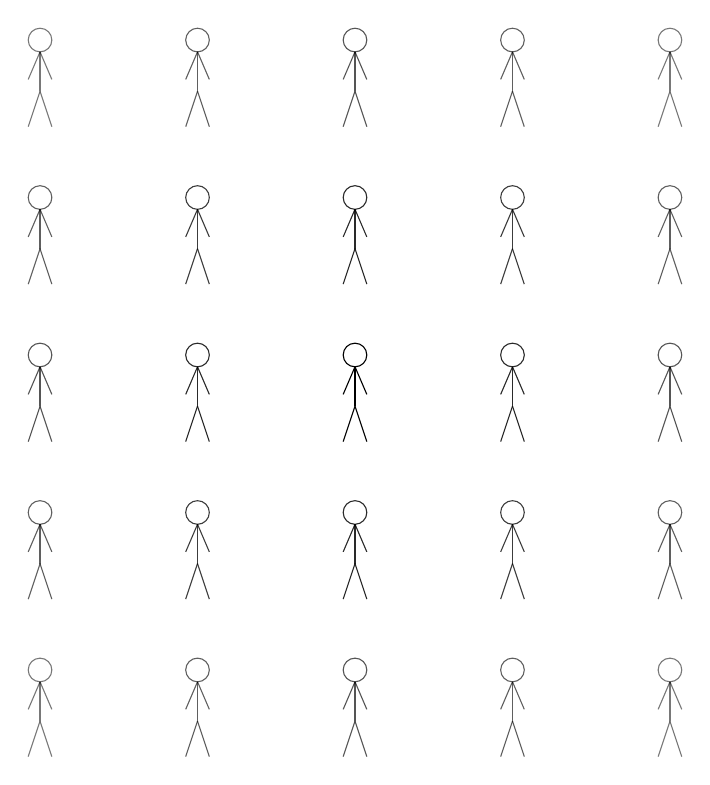
\begin{tikzpicture}
    \foreach \x in {-2,-1,...,2} {
      \foreach \y in {-2,-1,...,2} {
        \pgfmathsetmacro\c{1 - sqrt((\x)^2 + (\y)^2)/6};
        \begin{scope}[shift={(\x * 2, \y * 2)}, opacity=\c]
          \draw (0, 0.4) circle [radius=0.15];
          \draw (0, 0.25) -- (0, -0.25);
          \draw (0, -0.25) -- (-0.15, -0.7);
          \draw (0, -0.25) -- (0.15, -0.7);
          \draw (0, 0.25) -- (-0.15, -0.1);
          \draw (0, 0.25) -- (0.15, -0.1);
        \end{scope}
      }
    }
  \end{tikzpicture}
\end{center}
As we said, this looks somewhat likes $\R^2$, but we \emph{know} that this is not $\R^2$, since we can see some symmetry in this space. Whenever we move one unit horizontally or vertically, we get back to ``the same place''. In fact, we can move horizontally by $n$ units and vertically by $m$ units, for any $n, m \in \Z$, and still get back to the same place. This space has a huge translation symmetry. What is this symmetry? It is exactly $\Z \times \Z$.

We see that if we live inside the torus $S^1 \times S^1$, it feels like we are actually living in the universal covering space $\R \times \R$, except that we have an additional symmetry given by the fundamental group $\Z \times \Z$.

Hopefully, you are convinced that universal covers are nice. We would like to say that universal covers always exist. However, this is not always true.

Firstly, we should think --- what would having a universal cover imply? Suppose $X$ has a universal cover $\tilde{X}$. Pick any point $x_0 \in X$, and pick an evenly covered neighbourhood $U$ in $X$. This lifts to some $\tilde{U} \in \tilde{X}$. If we draw a teeny-tiny loop $\gamma$ around $x_0$ inside $U$, we can lift this $\gamma$ to $\tilde{\gamma}$ in $\tilde{U}$. But we know that $\tilde{X}$ is simply connected. So $\tilde{\gamma}$ is homotopic to the constant path. Hence $\gamma$ is also homotopic to the constant path. So all loops (contained in $U$) at $x_0$ are homotopic to the constant path.

It seems like for every $x_0 \in X$, there is some neighbourhood of $x_0$ that is simply connected. Except that's not what we just showed above. The homotopy from $\tilde{\gamma}$ to the constant path is a homotopy in $\tilde{X}$, and can pass through anything in $\tilde{X}$, not just $\tilde{U}$. Hence the homotopy induced in $X$ is also a homotopy in $X$, not a homotopy in $U$. So $U$ itself need not be simply connected. What we have is a slightly weaker notion.

\begin{defi}[Locally simply connected]
  $X$ is \emph{locally simply connected} if for all $x_0\in X$, there is some neighbourhood $U$ of $x_0$ such that $U$ is simply connected.
\end{defi}

As we mentioned, what we actually want is a weaker condition.
\begin{defi}[Semi-locally simply connected]
  $X$ is \emph{semi-locally simply connected} if for all $x_0 \in X$, there is some neighbourhood $U$ of $x_0$ such that any loop $\gamma$ based at $x_0$ is homotopic to $c_{x_0}$ as paths \emph{in $X$}.
\end{defi}

We have just argued that if a universal cover $p: \tilde{X} \to X$ exists, then $X$ is semi-locally simply connected. This is really not interesting, since we don't care if a space is semi-locally simply connected. What is important is that this is the other direction.

\begin{thm}
  If $X$ is path connected, locally path connected and semi-locally simply connected, then $X$ has a universal covering.
\end{thm}
Note that we can alternatively define a universal covering as a covering space of $X$ that is also a covering space of all other covers of $X$. If we use this definition, then we can prove this result easily using Zorn's lemma. However, that proof is not too helpful since it does not tell us where the universal covering comes from. Instead, we will provide a constructive proof (sketch) that will hopefully be more indicative of what universal coverings are like.

\begin{proof}(idea)
  We pick a basepoint $x_0 \in X$ for ourselves. Suppose we have a universal covering $\tilde{X}$. Then we have some $\tilde{x}_0$ in $\tilde{X}$. If we have any other point $\tilde{x} \in \tilde{X}$, since $\tilde{X}$ should be path connected, there is a path $\tilde{\alpha}: \tilde{x}_0 \to \tilde{x}$. If we have another path, then since $\tilde{X}$ is simply connected, then the paths are homotopic. Hence, we can identify each point in $\tilde{X}$ with a path from $\tilde{x}_0$, ie.
  \[
    \{\text{points of }\tilde{X}\} \longleftrightarrow \{\text{paths }\tilde{\alpha}\text{ from }\tilde{x}_0\in \tilde{X}\}/{\simeq}.
  \]
  This is not too helpful too, since we are defining $\tilde{X}$ in terms of things in $\tilde{X}$. However, by path lifting, we know that paths $\tilde{\alpha}$ from $\tilde{x}_0$ in $\tilde{X}$ biject with paths $\alpha$ from $x_0$ in $X$. Also, by homotopy lifting, homotopies of paths in $X$ can be lifted to homotopies of paths in $\tilde{X}$. So we have
  \[
    \{\text{points of }\tilde{X}\} \longleftrightarrow \{\text{paths }\alpha\text{ from }x_0 \in X\}/{\simeq}.
  \]
  So we can produce our $\tilde{X}$ by picking a basepoint $x_0 \in X$, and defining
  \[
    \tilde{X} = \{\text{paths }\alpha: I\to X\text{ such that }\alpha(0) = x_0\}/{\simeq}.
  \]
  The covering map $p: \tilde{X} \to X$ is given by $[\alpha] \mapsto \alpha(1)$.

  One then has to work hard to define the topology, and then show this is simply connected.
\end{proof}

\subsection{The Galois correspondence}
Recall that at the beginning, we wanted to establish a correspondence between covering spaces and fundamental groups. We have already established the result that covering maps are injective on $\pi_1$. Therefore, given a (based) covering space $p \to (\tilde{X}, \tilde{x}_0) \to (X, x_0)$, we can give a subgroup $p_*(\tilde{X}, \tilde{x}_0)\leq \pi_1(X, x_0)$. It turns out that as long as we define carefully what we mean for based covering spaces to be ``the same'', this is a one-to-one correspondence --- each subgroup corresponds to a covering space.

We can have the following table of correspondence:
\begin{center}
  \begin{tabular}{rcl}
    \textbf{Covering spaces} & $\longleftrightarrow$ & \textbf{Fundamental group}\\
    (Based) covering spaces & $\longleftrightarrow$ & Subgroups of $\pi_1$\\
    Degree & $\longleftrightarrow$ & Index\\
    Universal covers & $\longleftrightarrow$ & Trivial subgroup\\
  \end{tabular}
\end{center}
We now want to look at some of these correspondences.

Recall that we have shown that $\pi_1(X, x_0)$ acts on $p^{-1}(x_0)$. However, this is not a too interesting action, since $p^{-1}(x_0)$ is a discrete group with no structure. Having groups acting on a cube is fun because the cube has some structure. So we want something more ``rich'' for $\pi_1(X, x_0)$ to act on.

We note that we can make $\pi_1(X, x_0)$ ``act on'' the universal cover. How? Recall that in the torus example, each item in the fundamental group corresponds to translating the whole universal covering by some amount. In general, a point on $\tilde{X}$ can be thought of as a path $\alpha$ on $X$ starting from $x_0$. Then it is easy to make a loop $\gamma: x_0 \leadsto x_0$ act on this: use the composition $\gamma\cdot \alpha$: $[\gamma]\cdot [\alpha] = [\gamma \cdot \alpha]$.
\begin{center}
  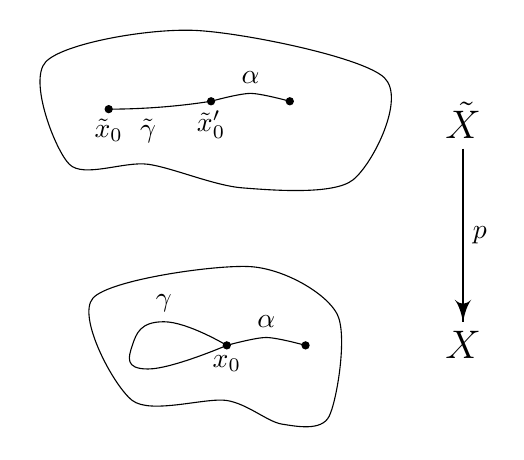
\begin{tikzpicture}
    \draw plot [smooth cycle] coordinates {(-1.2, -0.7) (0, -0.7) (0.7, -1) (1.3, -0.9) (1.4, 0.4) (0.3, 1) (-1.7, 0.6)};

    \begin{scope}[shift={(-1, 3)}]
      \draw plot [smooth cycle] coordinates {(-1, -0.7) (0, -0.7) (1.2, -1) (2.6, -0.9) (3, 0.4) (0.6, 1) (-1.3, 0.6)};
      \node [below] at (-0.5, 0) {$\tilde{x}_0$};
      \node [below] at (0.8, 0.1) {$\tilde{x}_0'$};
      \draw (-0.5, 0) parabola (0.8, 0.1) node [pos=0.5, below] {$\tilde{\gamma}$};

      \node [circ] at (-0.5, 0) {};
      \node [circ] at (0.8, 0.1) {};

      \draw plot [smooth] coordinates {(0.8, 0.1) (1.3, 0.2) (1.8, 0.1)};
      \node [circ] at (1.8, 0.1) {};
    \node [above] at (1.3, 0.2) {$\alpha$};
    \end{scope}

    \draw [->] (3, 2.5) node [above] {\Large $\tilde{X}$} -- +(0, -2.2) node [below] {\Large $X$} node [pos=0.5, right] {$p$};

    \node [circ] at (0, 0) {};
    \node [below] at (0, 0) {$x_0$};

    \draw plot [tension=0.9, smooth] coordinates {(0, 0) (-1, -0.3) (-1.2, 0) (-0.8, 0.3) (0, 0)};
    \node at (-0.8, 0.3) [above] {$\gamma$};

    \draw plot [smooth] coordinates {(0, 0) (0.5, 0.1) (1, 0)};
    \node [circ] at (1, 0) {};
    \node [above] at (0.5, 0.1) {$\alpha$};


  \end{tikzpicture}
\end{center}
We will use this idea and return to the initial issue of making subgroups correspond with covering spaces. We want to show that this is surjective --- every subgroup arises from some cover. We want to say ``For any subgroup $H \leq \pi_1(X, x_0)$, there is a based covering map $p: (\tilde{X}, \tilde{x}_0)\to (X, x_0)$ such that $p_* \pi_1(\tilde{X}, \tilde{x}_0) = H$''. Except, this cannot possibly be true, since by taking the trivial subgroup, this would imply that there is a universal covering for every space. So we need some additional assumptions.

\begin{prop}
  Let $X$ be a path connected, locally path connected and semi-locally simply connected space. For any subgroup $H \leq \pi_1(X, x_0)$, there is a based covering map $p: (\tilde{X}, \tilde{x}_0)\to (X, x_0)$ such that $p_* \pi_1(\tilde{X}, \tilde{x}_0) = H$>
\end{prop}

\begin{proof}
  Since $X$ is path connected, locally path connected and semi-locally simply connected space, let $\bar{X}$ be a universal covering. We have an intermediate group $H$ such that $\pi_1(\tilde{X}, \tilde{x}_0) = 1 \leq H \leq \pi_1(X, x_0)$. How can we obtain a corresponding covering space?

  Note that if we have $\bar{X}$ and we want to recover $X$, we can quotient $\bar{X}$ by the action of $\pi_1(X, x_0)$. Since $\pi_1(X, x_0)$ acts on $\bar{X}$, so does $H \leq \pi_1(X, x_0)$. Now we can define our covering space by taking quotients. We define $\sim_H$ on $\bar{X}$ to be the orbit relation for the action of $H$, ie. $\tilde{X} \sim_H \tilde{y}$ if there is some $h \in H$  such that $\tilde{y} = h\tilde{x}$. We then let $\tilde{X}$ be the quotient space $\bar{X}/{\sim_H}$.

  We can now do the messy algebra to show that this is the covering space we want.
\end{proof}
\end{document}
